\begin{figure}[ht]
\centering
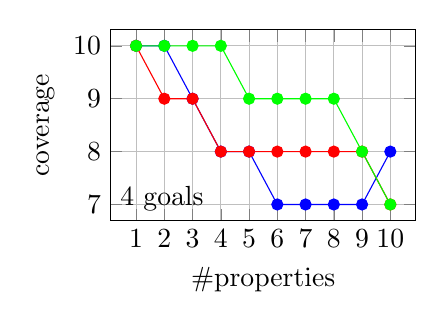
\begin{tikzpicture}
	\begin{axis}[
		title={4 goals},
		every axis title/.style={above right,at={(0,0)}},
		height=4cm,
		width=0.45\textwidth,
		xlabel=\#properties,
		ylabel=coverage,
		ytick={1,2,3,4,5,6,7,8,9,10},
		xtick={1,2,3,4,5,6,7,8,9,10},
		%xmin=0,
		%xmax=10,
		%ymin=0,
		%ymax=10,
		grid,
		%ybar,
		%bar width=2pt,
		legend style={at={(0.5,1.15)}, anchor=north,legend columns=-1},
		%mark options={%
		%	scale=2,fill=yellow!80!black,draw=black
		%}
	]
	\addplot+[blue,mark=*, mark options={fill=blue}] coordinates {
				(1,10) (2,10) (3,9) (4,8) (5,8) (6,7) (7,7) (8,7) (9,7) (10,8)
	};
	\addplot+[red,mark=*, mark options={fill=red}] coordinates {
				(1,10) (2,9) (3,9) (4,8) (5,8) (6,8) (7,8) (8,8) (9,8) (10,7)
	};
	\addplot+[green,mark=*, mark options={fill=green}] coordinates {
				(1,10) (2,10) (3,10) (4,10) (5,9) (6,9) (7,9) (8,9) (9,8) (10,7)
	};

	
	%\legend{hC, hC no reuse, hmax}
	\end{axis}
\end{tikzpicture}
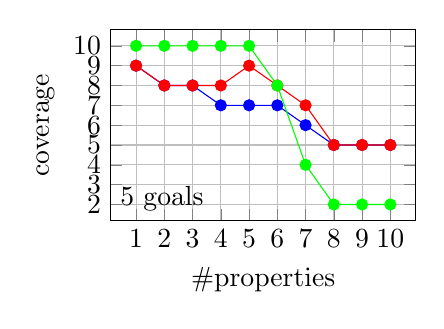
\begin{tikzpicture}
	\begin{axis}[
		title={5 goals},
		every axis title/.style={above right,at={(0,0)}},
		height=4cm,
		width=0.45\textwidth,
		xlabel=\#properties,
		ylabel=coverage,
		ytick={1,2,3,4,5,6,7,8,9,10},
		xtick={1,2,3,4,5,6,7,8,9,10},
		%xmin=0,
		%xmax=10,
		%ymin=0,
		%ymax=10,
		grid,
		%ybar,
		%bar width=2pt,
		legend style={at={(0.5,1.15)}, anchor=north,legend columns=-1},
		%mark options={%
		%	scale=2,fill=yellow!80!black,draw=black
		%}
	]
	\addplot+[blue, mark=*, mark options={fill=blue}] coordinates {
				(1,9) (2,8) (3,8) (4,7) (5,7) (6,7) (7,6) (8,5) (9,5) (10,5)
	};
	\addplot+[red, mark=*, mark options={fill=red}] coordinates {
				(1,9) (2,8) (3,8) (4,8) (5,9) (6,8) (7,7) (8,5) (9,5) (10,5)
	};
	\addplot+[green, mark=*, mark options={fill=green}] coordinates {
				(1,10) (2,10) (3,10) (4,10) (5,10) (6,8) (7,4) (8,2) (9,2) (10,2)
	};
	
	%\legend{hC, hC no reuse, hmax}
	\end{axis}
\end{tikzpicture}
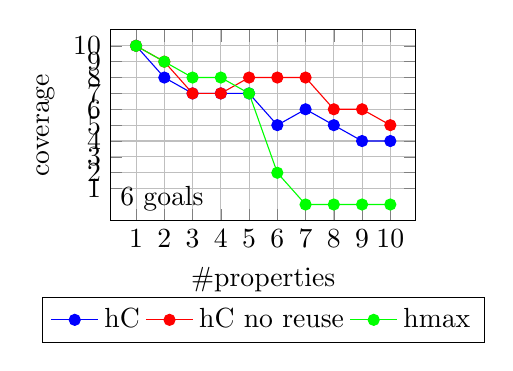
\begin{tikzpicture}
	\begin{axis}[
		title={6 goals},
		every axis title/.style={above right,at={(0,0)}},
		height=4cm,
		width=0.45\textwidth,
		xlabel=\#properties,
		ylabel=coverage,
		ytick={1,2,3,4,5,6,7,8,9,10},
		xtick={1,2,3,4,5,6,7,8,9,10},
		%xmin=0,
		%xmax=10,
		%ymin=0,
		%ymax=10,
		grid,
		%ybar,
		%bar width=2pt,
		legend style={at={(0.5,-0.4)}, anchor=north,legend columns=-1},
		%mark options={%
		%	scale=2,fill=yellow!80!black,draw=black
		%}
	]

	\addplot+[blue, mark=*, solid,mark options={fill=blue}] coordinates {
				(1,10) (2,8) (3,7) (4,7) (5,7) (6,5) (7,6) (8,5) (9,4) (10,4)
	};
	\addplot+[red, mark=*, mark options={fill=red}] coordinates {
				(1,10) (2,9) (3,7) (4,7) (5,8) (6,8) (7,8) (8,6) (9,6) (10,5)
	};
	\addplot+[green, mark=*, mark options={fill=green}] coordinates {
				(1,10) (2,9) (3,8) (4,8) (5,7) (6,2) (7,0) (8,0) (9,0) (10,0)
	};
	
	\legend{hC, hC no reuse, hmax}
	\end{axis}
\end{tikzpicture}
\caption{Comparison of coverage between the differenct heuristic functions in Nomystery domain with 2 trucks. Scale number of packages/goal facts between 4 and 6 and number of 
	properties between 1 and 10. The three property types blocked/forced road and two packages have
	to be delivered in the same truck are added in a fixed order. Meta search: top-down}
\end{figure}


\begin{figure}[ht]
\centering
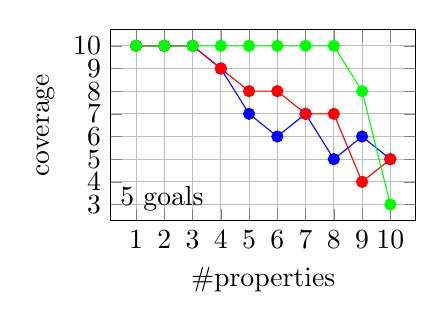
\begin{tikzpicture}
	\begin{axis}[
		title={5 goals},
		every axis title/.style={above right,at={(0,0)}},
		height=4cm,
		width=0.45\textwidth,
		xlabel=\#properties,
		ylabel=coverage,
		ytick={1,2,3,4,5,6,7,8,9,10},
		xtick={1,2,3,4,5,6,7,8,9,10},
		%xmin=0,
		%xmax=10,
		%ymin=0,
		%ymax=10,
		grid,
		%ybar,
		%bar width=2pt,
		legend style={at={(0.5,1.15)}, anchor=north,legend columns=-1},
	]
				
	\addplot+[blue,mark=*, mark options={fill=blue}] coordinates {
				(1,10) (2,10) (3,10) (4,9) (5,7) (6,6) (7,7) (8,5) (9,6) (10,5)
	};
	\addplot+[red,mark=*, mark options={fill=red}] coordinates {
				(1,10) (2,10) (3,10) (4,9) (5,8) (6,8) (7,7) (8,7) (9,4) (10,5)
	};
	\addplot+[green,mark=*, mark options={fill=green}] coordinates {
				(1,10) (2,10) (3,10) (4,10) (5,10) (6,10) (7,10) (8,10) (9,8) (10,3)
	};

	%\legend{hC, hC no reuse, hmax}
	\end{axis}
\end{tikzpicture}
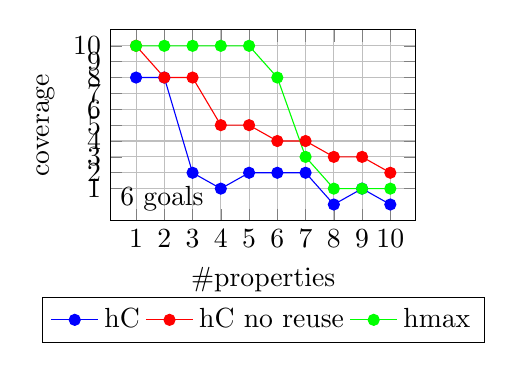
\begin{tikzpicture}
	\begin{axis}[
		title={6 goals},
		every axis title/.style={above right,at={(0,0)}},
		height=4cm,
		width=0.45\textwidth,
		xlabel=\#properties,
		ylabel=coverage,
		ytick={1,2,3,4,5,6,7,8,9,10},
		xtick={1,2,3,4,5,6,7,8,9,10},
		%xmin=0,
		%xmax=10,
		%ymin=0,
		%ymax=10,
		grid,
		%ybar,
		%bar width=2pt,
		legend style={at={(0.5,-0.4)}, anchor=north,legend columns=-1},
	]

	\addplot+[blue, mark=*, mark options={fill=blue}] coordinates {
				(1,8) (2,8) (3,2) (4,1) (5,2) (6,2) (7,2) (8,0) (9,1) (10,0)
	};
	\addplot+[red, mark=*, mark options={fill=red}] coordinates {
				(1,10) (2,8) (3,8) (4,5) (5,5) (6,4) (7,4) (8,3) (9,3) (10,2)
	};
	\addplot+[green, mark=*, mark options={fill=green}] coordinates {
				(1,10) (2,10) (3,10) (4,10) (5,10) (6,8) (7,3) (8,1) (9,1) (10,1)
	};

	
	\legend{hC, hC no reuse, hmax}
	\end{axis}
\end{tikzpicture}
\caption{Comparison of coverage between the different heuristic functions in the TPP domain with 2 trucks. Scale number of packages between 5 and 6 and number of 
	properties between 1 and 10. The three property types blocked/forced road and one goods needs to be bought a 
	specific market are added in a fixed order.  Meta search: top-down}
\end{figure}


\newpage
\begin{figure}[ht]
\small
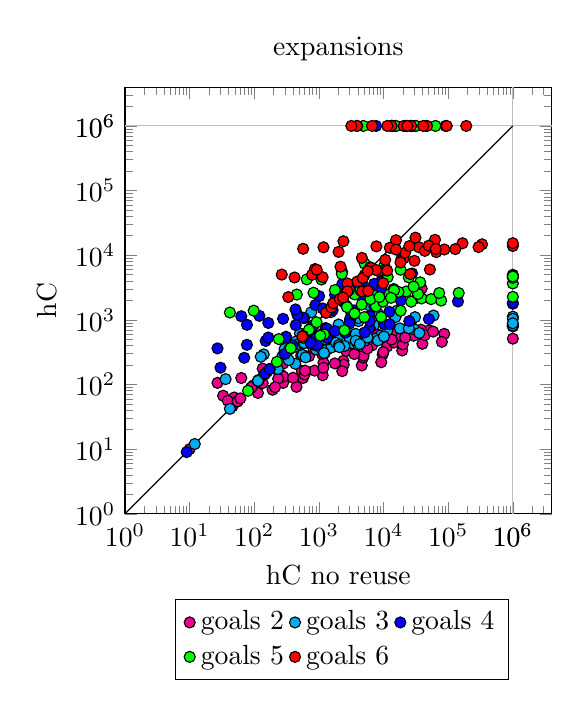
\begin{tikzpicture}
\begin{axis}[extra x tick style={grid=major},
	extra x ticks=1000000,
extra y tick style={grid=major},
extra y ticks=1000000,
height=7cm,
legend cell align=left,
legend style={at={(0.9,-0.2)}, legend columns=3},
title=expansions,
width=7cm,
xlabel=hC no reuse,
xmin=1,
xmode=log,
ylabel=hC, 
ymin=1, 
ymode=log]
\addplot[color=magenta, mark=*, mark options={{draw=black}}, only marks] coordinates {
(4599, 197) (51150, 688) (49, 63) (0.100000, 299) (1547, 436) (38874, 3047) (19418, 336) (9690, 290) (86870, 607) (39858, 426) (0.100000, 251) (279, 106) (11403, 389) (261, 140) (280, 133) (234, 123) (14535, 445) (27, 106) (450, 92) (37851, 704) (567, 126) (0.100000, 154) (192, 83) (43350, 581) (570, 158) (174, 174) (0.100000, 163) (97, 97) (1701, 400) (1178, 218) (1143, 139) (2394, 232) (2418, 203) (0.100000, 300) (4826, 261) (531, 281) (702, 274) (0.100000, 252) (1767, 212) (0.100000, 239) (46, 46) (0.100000, 71) (15555, 654) (855, 164) (0.100000, 59) (33, 67) (10, 10) (4914, 280) (9207, 221) (0.100000, 269) (819, 366) (6885, 505) (135, 176) (546, 162) (2015, 398) (3315, 382) (114, 74) (0.100000, 192) (1651, 444) (19890, 418) (58311, 658) (56, 56) (79794, 457) (2295, 161) (63, 126) (29127, 569) (9906, 317) (18907, 561) (1170, 181) (7112, 485) (28105, 751) (13299, 497) (0.100000, 301) (88, 88) (0.100000, 133) (21590, 532) (6643, 403) (54, 54) (5611, 360) (0.100000, 88) (39, 56) (55, 55) (144, 144) (600, 143) (3429, 457) (61, 61) (210, 91) (399, 127) (1239, 308) (1000000, 512) (279, 210) (1116, 297) (7747, 605) (609, 164) (2655, 330) (91, 91) (3843, 493) (975, 384) (3528, 296) (135, 105)
};
\addlegendentry{goals 2}
\addplot[color=cyan, mark=*, mark options={{draw=black}}, only marks] coordinates {
(432, 209) (3339, 433) (275, 275) (560, 287) (903, 347) (12, 12) (1000000, 799) (0.100000, 486) (5040, 473) (4092, 954) (7099, 833) (0.100000, 917) (343, 445) (1000000, 793) (1540, 371) (620, 454) (2044, 578) (30090, 707) (42, 42) (143, 143) (1530, 1317) (140, 292) (430, 430) (126, 269) (272, 272) (2970, 528) (3705, 608) (17885, 738) (3937, 444) (0.100000, 611) (113, 113) (1000000, 819) (2016, 847) (35805, 628) (300, 313) (1000000, 1120) (1386, 503) (0.100000, 195) (8925, 570) (11466, 689) (118, 118) (4064, 1062) (1000000, 1037) (620, 263) (885, 404) (0.100000, 345) (508, 618) (0.100000, 621) (294, 354) (4080, 407) (1829, 444) (0.100000, 866) (16352, 1399) (720, 671) (1099, 354) (0.100000, 205) (1008, 450) (2032, 407) (30660, 1101) (0.100000, 962) (231, 174) (6138, 1655) (762, 1312) (0.100000, 1875) (3024, 1436) (435, 460) (413, 378) (0.100000, 1946) (0.100000, 209) (0.100000, 432) (59334, 1167) (3717, 477) (7493, 510) (8176, 479) (15300, 1106) (32736, 2193) (5642, 533) (3066, 1425) (4278, 422) (1200, 307) (0.100000, 957) (10160, 553) (114, 114) (24552, 742) (0.100000, 731) (0.100000, 0.100000) (2480, 394) (0.100000, 718) (489, 424) (8160, 1255) (342, 238) (1000000, 885) (1260, 498) (36, 121) (157, 157) (1020, 578) (2070, 378) (576, 434) (594, 437) (1488, 658)
};
\addlegendentry{goals 3}
\addplot[color=blue, mark=*, mark options={{draw=black}}, only marks] coordinates {
(4704, 2113) (27621, 5220) (9198, 3946) (15330, 1000000) (0.100000, 473) (2412, 1900) (10230, 857) (1008, 2326) (376, 376) (165, 895) (903, 528) (0.100000, 266) (930, 409) (630, 614) (120, 1153) (1000000, 1777) (7223, 1606) (3060, 1009) (14322, 2997) (1270, 746) (749, 749) (12276, 1335) (27940, 1000000) (3024, 1031) (0.100000, 474) (63, 1138) (2550, 635) (1333, 727) (2286, 3224) (1631, 1413) (77, 411) (6107, 748) (4590, 3866) (6096, 1146) (7650, 1000000) (3570, 3272) (591, 1061) (738, 443) (769, 769) (0.100000, 695) (0.100000, 257) (0.100000, 944) (1778, 2422) (2295, 3568) (346, 346) (387, 407) (25019, 957) (0.100000, 173) (141547, 1923) (0.100000, 881) (310, 548) (279, 1038) (4599, 3621) (173, 173) (50235, 1029) (150, 472) (3495, 1398) (6132, 964) (567, 1080) (2955, 870) (837, 837) (465, 1190) (77, 839) (7154, 3606) (882, 1699) (0.100000, 282) (1000000, 1840) (434, 1451) (1143, 1501) (27, 362) (9, 9) (30, 182) (70, 259) (147, 147) (1335, 526) (296, 296) (1757, 674) (165, 533) (9207, 3015) (13860, 1000000) (18414, 2004) (172, 172) (438, 828) (12411, 854) (5110, 638)
};
\addlegendentry{goals 4}
\addplot[color=green, mark=*, mark options={{draw=black}}, only marks] coordinates {
(1095, 4212) (77748, 1986) (80, 80) (1286, 1286) (13175, 1000000) (98, 1387) (702, 702) (13104, 1000000) (38836, 2145) (91047, 1000000) (2275, 5588) (22695, 1000000) (224, 224) (42, 1300) (45479, 1000000) (0.100000, 1630) (1200, 596) (22413, 2751) (7239, 2370) (2263, 5137) (26753, 1909) (4585, 1723) (36828, 3806) (7650, 1618) (15500, 1000000) (2673, 1632) (12400, 2493) (24540, 4534) (11578, 4584) (455, 2462) (9144, 1112) (6258, 2089) (18360, 1382) (18333, 5966) (1767, 2891) (145266, 2602) (1473, 1473) (3591, 2473) (560, 529) (1000000, 2271) (1472, 1472) (1000000, 4977) (825, 2627) (1000000, 4830) (9825, 1914) (1000000, 3658) (366, 366) (4875, 1000000) (34170, 2517) (10287, 6890) (54369, 2090) (4383, 2877) (31496, 1000000) (240, 504) (17018, 2707) (1000000, 4472) (72562, 2602) (0.100000, 1921) (648, 4233) (14535, 2862) (13050, 2190) (63500, 1000000) (2595, 2595) (1000000, 4683) (2715, 1575) (8631, 2254) (31500, 1000000) (919, 919) (26416, 1000000) (29127, 3268) (5103, 7403) (2480, 688) (3570, 1254) (0.100000, 1637) (2910, 2910) (5040, 1102) (9486, 5730) (1050, 569)
};
\addlegendentry{goals 5}
\addplot[color=red, mark=*, mark options={{draw=black}}, only marks] coordinates {
(18900, 8717) (565, 565) (20305, 8903) (15555, 17047) (1292, 1292) (868, 6106) (333498, 14739) (420, 4528) (6223, 6507) (47117, 1000000) (35343, 13277) (1178, 13248) (40950, 1000000) (784, 4973) (1141, 4568) (1557, 1557) (1000000, 13893) (166586, 15317) (65405, 11183) (2016, 11258) (43434, 11665) (87210, 12266) (62403, 17312) (13286, 1000000) (6268, 6268) (21546, 10963) (570, 12572) (2156, 6648) (7747, 13704) (5085, 4922) (1000000, 15370) (4671, 2740) (25830, 5102) (25039, 13840) (3919, 3919) (4770, 4433) (3918, 1000000) (12495, 13014) (8400, 5672) (26598, 1000000) (6362, 6362) (7674, 5907) (52070, 6012) (2946, 2946) (266, 5011) (9858, 3709) (2394, 16457) (11439, 1000000) (30039, 8195) (1662, 1809) (3843, 1000000) (4620, 9099) (15562, 12215) (3175, 1000000) (924, 5952) (336, 2252) (20460, 1000000) (50127, 14064) (2769, 3652) (5691, 5691) (94860, 1000000) (31171, 18691) (294847, 13362) (554, 554) (10602, 8487) (5763, 2807) (64135, 12513) (2761, 2761) (18267, 7725) (23247, 1000000) (2104, 2104) (2359, 2208) (11389, 5776) (128775, 12433) (190092, 1000000) (6630, 1000000)
};
\addlegendentry{goals 6}
\addplot[color=black] coordinates {(0.050000, 0.050000) (1000000, 1000000)};
\end{axis}
\end{tikzpicture}

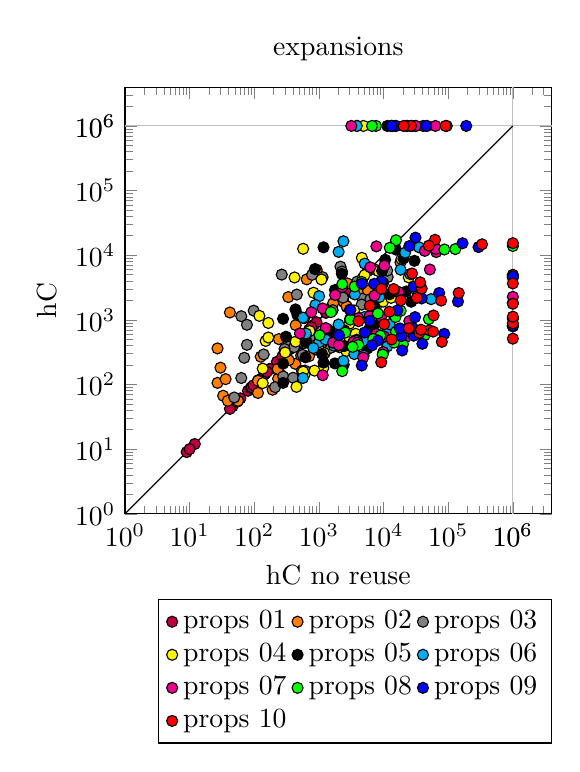
\begin{tikzpicture}
\begin{axis}[extra x tick style={grid=major},
	extra x ticks=1000000,
extra y tick style={grid=major},
extra y ticks=1000000,
height=7cm,
legend cell align=left,
legend style={at={(1.0,-0.2)}, legend columns=3},
title=expansions,
width=7cm,
xlabel=hC no reuse,
xmin=1,
xmode=log,
ylabel=hC,
ymin=1,
ymode=log]
\addplot[color=purple, mark=*, mark options={{draw=black}}, only marks] coordinates {
(144, 144) (1557, 1557) (1286, 1286) (12, 12) (275, 275) (55, 55) (113, 113) (80, 80) (376, 376) (6268, 6268) (702, 702) (554, 554) (172, 172) (565, 565) (147, 147) (837, 837) (61, 61) (46, 46) (346, 346) (0.100000, 0.100000) (174, 174) (919, 919) (224, 224) (430, 430) (2946, 2946) (2104, 2104) (42, 42) (143, 143) (1472, 1472) (6362, 6362) (366, 366) (749, 749) (9, 9) (1292, 1292) (88, 88) (173, 173) (5691, 5691) (157, 157) (91, 91) (2595, 2595) (54, 54) (118, 118) (2761, 2761) (769, 769) (296, 296) (272, 272) (2910, 2910) (97, 97) (10, 10)
};
\addlegendentry{props 01}
\addplot[color=orange, mark=*, mark options={{draw=black}}, only marks] coordinates {
(432, 209) (2412, 1900) (648, 4233) (56, 56) (42, 1300) (930, 409) (30, 182) (4383, 2877) (261, 140) (0.100000, 205) (531, 281) (234, 123) (114, 114) (4671, 2740) (438, 828) (591, 1061) (738, 443) (1473, 1473) (3918, 1000000) (231, 174) (387, 407) (489, 424) (924, 5952) (0.100000, 173) (342, 238) (2715, 1575) (27, 106) (33, 67) (36, 121) (240, 504) (7674, 5907) (2769, 3652) (336, 2252) (702, 274) (27, 362) (1000000, 1840) (5763, 2807) (192, 83) (39, 56) (576, 434) (18267, 7725) (126, 269) (594, 437) (1662, 1809) (2673, 1632) (1050, 569) (114, 74)
};
\addlegendentry{props 02}
\addplot[color=gray, mark=*, mark options={{draw=black}}, only marks] coordinates {
(4704, 2113) (560, 287) (903, 347) (280, 133) (140, 292) (1547, 436) (63, 126) (77, 411) (784, 4973) (1141, 4568) (1239, 308) (4585, 1723) (63, 1138) (1099, 354) (343, 445) (98, 1387) (399, 127) (2156, 6648) (3570, 1254) (11578, 4584) (455, 2462) (77, 839) (6258, 2089) (2359, 2208) (210, 91) (3919, 3919) (11389, 5776) (560, 529) (1540, 371) (266, 5011) (2275, 5588) (609, 164) (1386, 503) (0.100000, 195) (49, 63) (413, 378) (0.100000, 59) (0.100000, 282) (1631, 1413) (70, 259) (294, 354) (1757, 674) (546, 162) (903, 528)
};
\addlegendentry{props 03}
\addplot[color=yellow, mark=*, mark options={{draw=black}}, only marks] coordinates {
(1095, 4212) (18900, 8717) (885, 404) (165, 895) (150, 472) (0.100000, 345) (8400, 5672) (600, 143) (420, 4528) (570, 12572) (0.100000, 266) (120, 1153) (2970, 528) (1200, 307) (720, 671) (7650, 1618) (24540, 4534) (2655, 330) (1170, 181) (825, 2627) (4770, 4433) (9825, 1914) (4875, 1000000) (300, 313) (0.100000, 71) (435, 460) (4620, 9099) (1200, 596) (3495, 1398) (5085, 4922) (2955, 870) (855, 164) (13050, 2190) (450, 92) (2070, 378) (975, 384) (0.100000, 209) (1335, 526) (3705, 608) (570, 158) (135, 176) (165, 533) (135, 105)
};
\addlegendentry{props 04}
\addplot[color=black, mark=*, mark options={{draw=black}}, only marks] coordinates {
(1178, 218) (13175, 1000000) (1178, 13248) (0.100000, 621) (868, 6106) (5642, 533) (4278, 422) (7223, 1606) (22413, 2751) (2418, 203) (1829, 444) (2263, 5137) (26753, 1909) (9858, 3709) (2015, 398) (279, 106) (20305, 8903) (620, 263) (1333, 727) (12400, 2493) (15562, 12215) (1767, 2891) (434, 1451) (279, 210) (1767, 212) (2480, 688) (465, 1190) (2480, 394) (1116, 297) (6107, 748) (620, 454) (11439, 1000000) (30039, 8195) (279, 1038) (7099, 833) (0.100000, 133) (0.100000, 257) (15500, 1000000) (310, 548) (10602, 8487) (0.100000, 88) (5611, 360) (0.100000, 432) (9486, 5730) (1488, 658)
};
\addlegendentry{props 05}
\addplot[color=cyan, mark=*, mark options={{draw=black}}, only marks] coordinates {
(3339, 433) (1701, 400) (0.100000, 486) (35343, 13277) (630, 614) (5040, 473) (1000000, 4830) (13860, 1000000) (2016, 11258) (11403, 389) (567, 1080) (21546, 10963) (1008, 450) (8631, 2254) (54369, 2090) (25830, 5102) (3591, 2473) (0.100000, 731) (2016, 847) (2394, 16457) (3024, 1436) (18333, 5966) (3528, 296) (3843, 1000000) (40950, 1000000) (1008, 2326) (3024, 1031) (0.100000, 474) (567, 126) (882, 1699) (0.100000, 154) (11466, 689) (2394, 232) (1260, 498) (4914, 280) (3843, 493) (819, 366) (13104, 1000000) (23247, 1000000) (5103, 7403) (5040, 1102) (0.100000, 163) (31500, 1000000) (3717, 477) (12411, 854)
};
\addlegendentry{props 06}
\addplot[color=magenta, mark=*, mark options={{draw=black}}, only marks] coordinates {
(7493, 510) (0.100000, 192) (1651, 444) (4826, 261) (0.100000, 473) (1143, 139) (6223, 6507) (0.100000, 299) (7239, 2370) (3429, 457) (27940, 1000000) (43434, 11665) (762, 1312) (2286, 3224) (2032, 407) (7747, 13704) (9906, 317) (9144, 1112) (6096, 1146) (3937, 444) (0.100000, 718) (0.100000, 611) (1270, 746) (7112, 485) (1000000, 2271) (1778, 2422) (1000000, 4977) (10160, 553) (52070, 6012) (10287, 6890) (31496, 1000000) (3175, 1000000) (65405, 11183) (17018, 2707) (25019, 957) (21590, 532) (64135, 12513) (1000000, 793) (1143, 1501) (508, 618) (47117, 1000000) (26416, 1000000) (4064, 1062) (7747, 605) (63500, 1000000)
};
\addlegendentry{props 07}
\addplot[color=green, mark=*, mark options={{draw=black}}, only marks] coordinates {
(1000000, 799) (7650, 1000000) (19890, 418) (15555, 17047) (2295, 161) (22695, 1000000) (3060, 1009) (0.100000, 866) (1000000, 13893) (0.100000, 251) (87210, 12266) (2550, 635) (8925, 570) (4080, 407) (9690, 290) (15300, 1106) (3570, 3272) (14535, 445) (0.100000, 962) (0.100000, 695) (1000000, 4472) (12495, 13014) (2295, 3568) (18360, 1382) (34170, 2517) (8160, 1255) (1020, 578) (50235, 1029) (6630, 1000000) (30090, 707) (15555, 654) (14535, 2862) (0.100000, 269) (43350, 581) (6885, 505) (1530, 1317) (4590, 3866) (0.100000, 1637) (128775, 12433) (94860, 1000000) (3315, 382)
};
\addlegendentry{props 08}
\addplot[color=blue, mark=*, mark options={{draw=black}}, only marks] coordinates {
(9198, 3946) (15330, 1000000) (8176, 479) (38836, 2145) (4599, 197) (3066, 1425) (45479, 1000000) (19418, 336) (0.100000, 300) (86870, 607) (16352, 1399) (39858, 426) (166586, 15317) (4599, 3621) (13286, 1000000) (0.100000, 1875) (29127, 569) (30660, 1101) (18907, 561) (17885, 738) (31171, 18691) (0.100000, 957) (72562, 2602) (25039, 13840) (1000000, 819) (0.100000, 239) (28105, 751) (141547, 1923) (0.100000, 881) (2044, 578) (6132, 964) (6643, 403) (0.100000, 1921) (7154, 3606) (1000000, 4683) (294847, 13362) (29127, 3268) (1000000, 1037) (190092, 1000000) (5110, 638)
};
\addlegendentry{props 09}
\addplot[color=red, mark=*, mark options={{draw=black}}, only marks] coordinates {
(27621, 5220) (51150, 688) (1000000, 15370) (10230, 857) (58311, 658) (32736, 2193) (91047, 1000000) (79794, 457) (0.100000, 1630) (38874, 3047) (4092, 954) (333498, 14739) (12276, 1335) (0.100000, 917) (36828, 3806) (62403, 17312) (26598, 1000000) (1000000, 512) (24552, 742) (9207, 3015) (0.100000, 252) (1000000, 1777) (77748, 1986) (6138, 1655) (1000000, 3658) (35805, 628) (13299, 497) (0.100000, 301) (1000000, 885) (1000000, 1120) (14322, 2997) (20460, 1000000) (50127, 14064) (145266, 2602) (37851, 704) (0.100000, 1946) (9207, 221) (0.100000, 944) (18414, 2004) (59334, 1167)
};
\addlegendentry{props 10}
\addplot[color=black] coordinates {(0.050000, 0.050000) (1000000, 1000000)};
\end{axis}
\end{tikzpicture}

\caption{Comparison expansions per task in nomystery. hC: propagates the learned heuristic down the meta search tree, hC no reuse: computes the heuristic for every meta search node from scratch}
\end{figure}
\begin{figure}[ht]
\small
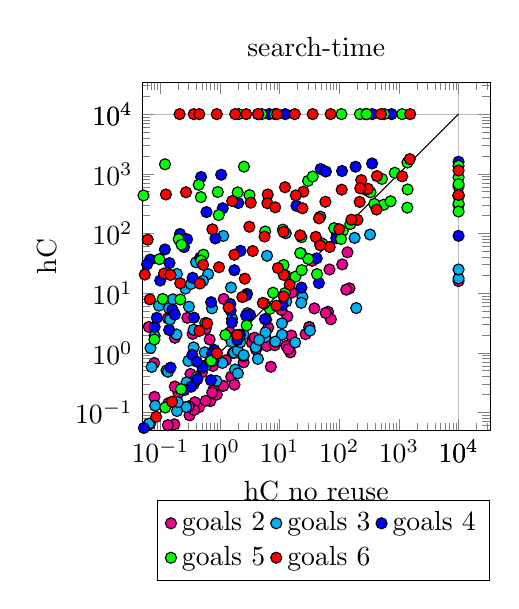
\begin{tikzpicture}
\begin{axis}[extra x tick style={grid=major},
	extra x ticks=10000,
extra y tick style={grid=major},
extra y ticks=10000,
height=6cm,
legend cell align=left,
legend style={at={(1.0,-0.2)}, legend columns=3},
title=search-time,
width=6cm,
xlabel=hC no reuse,
xmin=0.05,
xmode=log,
ylabel=hC,
ymin=0.05,
ymode=log]
\addplot[color=magenta, mark=*, mark options={{draw=black}}, only marks] coordinates {
(15.172100, 1.016770) (0.349230, 2.073010) (64.865700, 4.871180) (0.010059, 0.064839) (0.070098, 0.027386) (0.445538, 0.122297) (148.425000, 12.037600) (0.067012, 0.063801) (2.495880, 0.689987) (0.040536, 0.014467) (131.133000, 11.424200) (0.022867, 0.021803) (0.690293, 0.154804) (3.435980, 1.473070) (12.958100, 1.305790) (0.201632, 0.046902) (0.762613, 0.602015) (0.380498, 0.148276) (0.225019, 0.045287) (0.021991, 0.475112) (1.893380, 1.011710) (0.041468, 0.024021) (1.649410, 0.987147) (0.010000, 0.010000) (0.010149, 0.051998) (0.080068, 0.182478) (0.041789, 0.180893) (0.032815, 0.029216) (72.455800, 3.640430) (0.310373, 0.089486) (13.545500, 4.064030) (0.672865, 1.670940) (0.133950, 3.786150) (0.092355, 0.040271) (10000, 15.913400) (0.089941, 0.014108) (1.254740, 0.747294) (0.042804, 0.790036) (38.356300, 5.551290) (68.476800, 24.905900) (0.578483, 0.156651) (0.176234, 1.783280) (0.088824, 0.040993) (7.144020, 0.583110) (0.010000, 0.041604) (0.798899, 0.257890) (0.021901, 0.016696) (1.546940, 0.397283) (31.496300, 2.710360) (35.162100, 34.801600) (15.990900, 10.187200) (0.201670, 0.212821) (0.832051, 0.786923) (27.227300, 2.050610) (0.010000, 0.039432) (1.752980, 0.292273) (137.375000, 48.300900) (0.577804, 2.532230) (13.961800, 1.154880) (1.460960, 2.203480) (0.368463, 0.110043) (0.011319, 0.010497) (0.042066, 0.042300) (0.010000, 0.029778) (0.020331, 0.036438) (3.808380, 1.793480) (0.010000, 0.046530) (2.478070, 0.875246) (0.320369, 0.441322) (0.885287, 0.199093) (0.743278, 0.215247) (10.731100, 5.230970) (0.174990, 0.271837) (0.136985, 0.142653) (0.172666, 0.063263) (0.010000, 0.027149) (0.134334, 0.061225) (0.042038, 0.042319) (6.127500, 1.301100) (1.143180, 0.279111) (0.284799, 3.854150) (0.064472, 2.709750) (8.290520, 1.337350) (0.023067, 0.209633) (0.079221, 0.673988) (1.159620, 7.984760) (0.300164, 0.126549) (15.716800, 1.948390) (31.502700, 2.677360) (59.269800, 4.638450) (112.487000, 30.283700) (0.498080, 0.467415) (0.364356, 0.298650) (4.040940, 1.132660) (0.010588, 0.031236) (6.443390, 2.635040)
};
\addlegendentry{goals 2}
\addplot[color=cyan, mark=*, mark options={{draw=black}}, only marks] coordinates {
(5.970180, 3.601370) (1.597860, 3.706610) (0.018971, 0.589815) (0.264085, 11.902600) (0.080605, 1.921550) (0.271857, 0.123286) (1.138720, 91.003900) (0.326576, 14.250900) (0.403473, 0.389249) (0.190945, 0.105747) (5.757070, 1.835860) (6.162710, 42.257200) (328.832000, 95.791300) (0.010000, 0.156740) (24.156300, 8.594440) (10.945700, 3.108910) (10000, 421.288000) (0.010000, 0.098245) (0.010000, 0.010000) (0.558158, 1.016700) (0.870809, 0.338208) (0.068727, 1.202790) (193.148000, 5.620610) (0.363279, 1.232180) (1.723490, 1.007600) (0.739291, 5.548510) (0.023933, 3.674430) (4.335690, 0.788289) (0.146012, 3.613830) (0.363129, 2.435280) (0.582762, 0.618163) (0.296246, 0.729241) (0.010000, 0.335779) (1.536470, 12.417100) (12.943100, 7.252260) (0.634671, 20.753800) (32.351200, 2.359820) (0.030228, 0.449204) (1.991130, 1.103920) (180.929000, 84.350000) (0.190260, 20.931800) (10000, 17.631300) (1.100450, 0.675773) (0.520032, 16.037800) (0.011796, 2.082450) (2.849910, 9.704610) (2.998300, 4.229590) (0.071768, 0.578565) (102.785000, 86.321500) (10000, 24.921600) (3.994010, 1.242650) (0.027764, 0.025795) (10000, 426.467000) (0.037666, 1.128590) (0.041797, 0.574392) (5.816120, 2.195320) (10000, 299.098000) (0.277009, 0.319800) (0.095206, 6.168560) (0.187384, 2.032850) (47.679800, 70.182000) (0.303065, 5.915980) (0.036466, 0.038221) (0.029081, 0.029566) (12.684100, 100.741000) (1.519630, 1.751330) (22.847100, 46.682600) (0.010000, 0.169969) (1.568700, 1.524820) (0.196832, 0.148835) (0.064637, 0.064888) (0.139855, 5.590530) (1.795920, 0.523896) (2.496350, 2.031780) (12.561200, 19.756100) (48.211100, 191.367000) (18.267600, 1.484380) (0.398983, 32.884800) (0.082064, 0.129884) (10.979700, 2.007440) (8.453250, 1.540700) (0.163600, 7.865820) (0.127568, 0.505689) (0.019004, 0.603834) (2.501830, 0.915549) (2.900230, 4.604120) (4.540430, 1.640200) (2.193440, 1.497100) (23.097900, 6.875220) (0.041402, 0.037368) (2.001960, 0.451320) (0.017396, 0.422121) (0.805968, 0.934597) (0.010000, 0.766183) (10000, 437.903000) (0.046635, 3.883920) (0.010000, 0.060931) (0.134940, 0.481079)
};
\addlegendentry{goals 3}
\addplot[color=blue, mark=*, mark options={{draw=black}}, only marks] coordinates {
(111.578000, 1112.170000) (0.483449, 881.462000) (0.041698, 0.565731) (0.053170, 0.054861) (5.682950, 3.667030) (0.045937, 2.762800) (0.250826, 59.189100) (187.882000, 1314.830000) (0.010000, 0.013659) (0.330710, 0.269976) (0.214545, 98.012900) (0.067920, 36.489500) (0.010000, 19.455100) (2.168570, 2.004900) (41.880800, 38.315300) (1.963240, 1.646300) (10000, 91.178800) (0.020555, 0.474372) (0.027303, 38.337600) (0.802161, 1.117860) (3.198220, 4.324180) (0.011383, 2.681260) (0.010257, 0.350592) (0.466693, 39.107300) (0.024021, 7.626080) (0.704304, 0.347476) (0.160224, 5.312010) (0.141004, 2.411990) (0.143022, 31.843400) (2.748930, 4.213310) (0.281518, 79.956300) (89.307300, 83.310200) (355.338000, 1488.260000) (45.511000, 14.756000) (0.595686, 228.109000) (0.060081, 30.313200) (0.039189, 2.174940) (1.493130, 6.590090) (10000, 1589.450000) (0.148769, 0.563500) (0.010000, 0.458568) (0.099826, 16.242000) (0.119511, 53.933200) (2.215870, 51.124100) (0.080510, 2.716180) (282.027000, 536.002000) (0.010000, 0.473706) (1.748880, 24.188500) (23.240700, 12.365700) (0.020069, 0.554072) (48.856600, 1203.480000) (0.419938, 0.361739) (59.763800, 1091.030000) (0.254392, 0.237958) (12.421300, 10000) (90.049300, 105.897000) (1.116760, 264.395000) (0.020760, 1.199690) (0.010000, 0.489270) (2.774170, 9.167420) (1.514630, 5.111220) (11.168800, 6.334150) (358.113000, 10000) (0.344861, 0.919952) (0.348972, 18.088400) (0.010000, 0.330351) (753.841000, 10000) (2.029160, 324.059000) (0.712821, 7.039940) (0.012376, 0.014726) (0.011650, 0.418991) (1.051360, 964.510000) (0.513147, 0.570060) (0.010000, 0.985458) (0.410637, 0.709818) (19.146300, 290.395000) (6.700340, 10000) (1.589620, 3.229030) (0.175822, 4.368130) (0.010000, 0.010000) (0.738803, 0.973741) (0.368051, 3.880080) (0.780594, 0.734608) (0.087680, 3.860990) (0.841327, 82.488800)
};
\addlegendentry{goals 4}
\addplot[color=green, mark=*, mark options={{draw=black}}, only marks] coordinates {
(271.222000, 10000) (222.362000, 10000) (0.052377, 433.493000) (114.788000, 110.049000) (0.079793, 1.669360) (0.479611, 407.124000) (2.808070, 2.876580) (555.665000, 302.797000) (30.065800, 761.453000) (385.884000, 312.379000) (30.218400, 37.503700) (0.121296, 0.121056) (4.999540, 10000) (0.203565, 80.466600) (10000, 317.517000) (18.382400, 18.865000) (0.018612, 1.015510) (0.109973, 7.992210) (2.052910, 10000) (35.903400, 898.927000) (0.010000, 0.342310) (0.922682, 494.859000) (299.950000, 541.250000) (10000, 1362.290000) (0.528951, 44.038100) (11.353000, 115.888000) (725.921000, 345.763000) (107.176000, 80.746700) (0.044036, 1.627270) (7.765510, 10.157800) (5.743120, 107.795000) (10000, 232.750000) (108.740000, 10000) (334.567000, 490.006000) (0.120262, 1443.530000) (23.496800, 24.271100) (0.481242, 35.126400) (292.437000, 10000) (42.446200, 20.830300) (23.288600, 86.487500) (6.870990, 5.440640) (11.663800, 29.608800) (852.681000, 1039.820000) (0.441987, 654.423000) (0.096874, 37.078300) (2.533150, 1317.830000) (1383.430000, 270.944000) (1.985810, 487.783000) (1.235040, 1.992840) (52.738600, 66.421800) (8.306000, 10000) (153.562000, 143.760000) (10000, 872.787000) (10000, 614.469000) (287.088000, 10000) (0.024576, 2.173670) (1135.500000, 10000) (3.128460, 439.166000) (0.010000, 25.699500) (10000, 669.585000) (0.227354, 64.725200) (0.216906, 7.808270) (0.955310, 203.538000) (1399.870000, 546.159000) (519.330000, 820.633000) (0.568523, 3.161760) (0.692473, 0.733357) (0.711577, 0.735422) (22.194800, 46.798400) (0.010000, 42.995100) (567.899000, 10000) (4.344800, 10000) (0.010000, 0.010000) (1390.460000, 1543.890000) (5.583270, 6.701520) (12.332700, 10.026900) (0.222593, 0.245547) (82.358900, 122.731000)
};
\addlegendentry{goals 5}
\addplot[color=red, mark=*, mark options={{draw=black}}, only marks] coordinates {
(24.176300, 264.244000) (3.549660, 50.744900) (11.637800, 106.141000) (202.269000, 168.993000) (3.285440, 327.808000) (0.124485, 449.932000) (0.891800, 0.978837) (69.192800, 59.306700) (0.085376, 0.084345) (58.610600, 339.693000) (99.595500, 117.860000) (8.818960, 6.151750) (1.608570, 348.936000) (1542.990000, 10000) (40.433700, 87.685500) (499.524000, 10000) (0.115778, 21.322900) (12.338200, 594.863000) (0.364997, 10000) (6.332060, 449.164000) (2.378400, 8.599030) (220.006000, 337.925000) (10000, 442.115000) (0.966313, 27.139000) (0.029676, 92.075000) (1520.650000, 1763.810000) (0.522982, 29.822300) (10000, 1135.750000) (303.454000, 560.215000) (14.752000, 13.856500) (6.254180, 321.443000) (17.951200, 10000) (11.742000, 20.206400) (0.452037, 2.327490) (4.384470, 10000) (0.612628, 3.103410) (0.270357, 490.373000) (233.974000, 784.137000) (0.216657, 14.607900) (0.461476, 14.442700) (1.802090, 10000) (3.118740, 129.531000) (35.911600, 10000) (45.676200, 179.058000) (160.223000, 170.076000) (11.734500, 8.785160) (2.611100, 17.452900) (0.748514, 117.231000) (1.746640, 43.911800) (422.521000, 251.553000) (0.066958, 7.845780) (428.715000, 916.027000) (0.886132, 10000) (8.444990, 274.110000) (0.055071, 20.423400) (1134.970000, 905.843000) (0.450812, 10000) (1.945700, 1.989700) (25.097300, 500.616000) (18.708500, 434.721000) (0.061679, 78.629700) (110.004000, 541.935000) (1.397380, 5.736140) (225.165000, 570.223000) (9.383880, 26.309300) (22.193600, 93.209200) (0.013622, 5.685980) (71.711400, 10000) (2.761370, 10000) (5.593780, 88.646400) (5.240190, 6.834910) (48.129800, 63.152500) (0.210943, 10000) (9.109750, 10000) (0.148535, 20.155100) (0.157602, 0.151291)
};
\addlegendentry{goals 6}
\addplot[color=black] coordinates {(0.050000, 0.050000) (10000, 10000)};
\end{axis}
\end{tikzpicture}

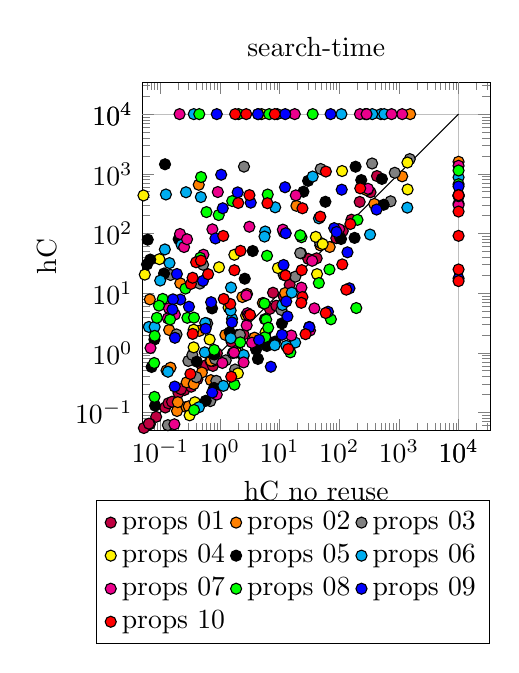
\begin{tikzpicture}
\begin{axis}[extra x tick style={grid=major},
	extra x ticks=10000,
extra y tick style={grid=major},
extra y ticks=10000,
height=6cm,
legend cell align=left,
legend style={at={(1.0,-0.2)}}, legend columns=3,
title=search-time,
width=6cm,
xlabel=hC no reuse,
xmin=0.05,
xmode=log,
ylabel=hC,
ymin=0.05,
ymode=log]
\addplot[color=purple, mark=*, mark options={{draw=black}}, only marks] coordinates {
(0.513147, 0.570060) (0.053170, 0.054861) (114.788000, 110.049000) (0.029081, 0.029566) (0.085376, 0.084345) (41.880800, 38.315300) (1.963240, 1.646300) (0.121296, 0.121056) (6.870990, 5.440640) (0.582762, 0.618163) (428.715000, 916.027000) (8.818960, 6.151750) (0.419938, 0.361739) (0.011319, 0.010497) (220.006000, 337.925000) (0.042066, 0.042300) (89.307300, 83.310200) (7.765510, 10.157800) (334.567000, 490.006000) (0.067012, 0.063801) (0.042038, 0.042319) (160.223000, 170.076000) (11.734500, 8.785160) (0.022867, 0.021803) (0.041402, 0.037368) (0.254392, 0.237958) (0.891800, 0.978837) (0.762613, 0.602015) (0.036466, 0.038221) (0.330710, 0.269976) (1.945700, 1.989700) (0.012376, 0.014726) (0.136985, 0.142653) (1.568700, 1.524820) (0.201670, 0.212821) (0.692473, 0.733357) (0.064637, 0.064888) (0.222593, 0.245547) (0.010000, 0.010000) (14.752000, 13.856500) (2.496350, 2.031780) (0.157602, 0.151291) (30.218400, 37.503700)
};
\addlegendentry{props 01}
\addplot[color=orange, mark=*, mark options={{draw=black}}, only marks] coordinates {
(3.808380, 1.793480) (0.216657, 14.607900) (0.010000, 0.013659) (69.192800, 59.306700) (0.070098, 0.027386) (0.032815, 0.029216) (0.027764, 0.025795) (1542.990000, 10000) (0.010000, 0.342310) (299.950000, 541.250000) (0.704304, 0.347476) (2.378400, 8.599030) (0.141004, 2.411990) (0.127568, 0.505689) (0.271857, 0.123286) (0.010000, 0.029778) (0.277009, 0.319800) (0.300164, 0.126549) (10000, 1589.450000) (0.148769, 0.563500) (0.190945, 0.105747) (282.027000, 536.002000) (0.441987, 654.423000) (385.884000, 312.379000) (0.498080, 0.467415) (1.235040, 1.992840) (0.010000, 0.041604) (0.364356, 0.298650) (0.010000, 0.985458) (1134.970000, 905.843000) (0.010000, 25.699500) (22.847100, 46.682600) (0.010000, 0.330351) (0.780594, 0.734608) (0.010000, 0.098245) (0.066958, 7.845780) (0.196832, 0.148835) (0.711577, 0.735422) (19.146300, 290.395000) (0.452037, 2.327490) (0.010000, 0.010000) (5.240190, 6.834910) (48.129800, 63.152500) (0.010000, 0.060931) (2.849910, 9.704610) (12.332700, 10.026900)
};
\addlegendentry{props 02}
\addplot[color=gray, mark=*, mark options={{draw=black}}, only marks] coordinates {
(0.040536, 0.014467) (0.010000, 19.455100) (2.168570, 2.004900) (0.018612, 1.015510) (18.382400, 18.865000) (0.296246, 0.729241) (0.011383, 2.681260) (0.010257, 0.350592) (0.092355, 0.040271) (0.019004, 0.603834) (725.921000, 345.763000) (48.856600, 1203.480000) (355.338000, 1488.260000) (1520.650000, 1763.810000) (0.522982, 29.822300) (0.010000, 0.489270) (0.187384, 2.032850) (0.134334, 0.061225) (47.679800, 70.182000) (1.991130, 1.103920) (0.461476, 14.442700) (1.254740, 0.747294) (11.742000, 20.206400) (852.681000, 1039.820000) (2.533150, 1317.830000) (0.344861, 0.919952) (0.690293, 0.154804) (0.017396, 0.422121) (0.024576, 2.173670) (0.403473, 0.389249) (0.612628, 3.103410) (0.010000, 0.473706) (10.731100, 5.230970) (0.010000, 0.169969) (0.010000, 0.039432) (0.010000, 0.027149) (0.013622, 5.685980) (0.832051, 0.786923) (22.194800, 46.798400) (0.010000, 42.995100) (0.010000, 0.010000) (0.870809, 0.338208) (1.795920, 0.523896) (0.148535, 20.155100)
};
\addlegendentry{props 03}
\addplot[color=yellow, mark=*, mark options={{draw=black}}, only marks] coordinates {
(111.578000, 1112.170000) (0.363279, 1.232180) (40.433700, 87.685500) (102.785000, 86.321500) (0.010000, 0.458568) (0.010059, 0.064839) (4.999540, 10000) (0.363129, 2.435280) (0.310373, 0.089486) (0.027303, 38.337600) (0.041797, 0.574392) (0.010000, 0.335779) (9.383880, 26.309300) (5.816120, 2.195320) (0.966313, 27.139000) (2.748930, 4.213310) (0.030228, 0.449204) (42.446200, 20.830300) (0.024021, 7.626080) (2.478070, 0.875246) (0.089941, 0.014108) (0.672865, 1.670940) (0.096874, 37.078300) (0.020760, 1.199690) (0.020069, 0.554072) (0.029676, 92.075000) (52.738600, 66.421800) (0.010000, 0.046530) (1.746640, 43.911800) (0.052377, 433.493000) (0.021901, 0.016696) (0.055071, 20.423400) (0.201632, 0.046902) (0.010000, 0.156740) (0.044036, 1.627270) (1.397380, 5.736140) (0.380498, 0.148276) (1399.870000, 546.159000) (1.893380, 1.011710) (3.994010, 1.242650) (0.738803, 0.973741) (2.001960, 0.451320) (1390.460000, 1543.890000)
};
\addlegendentry{props 04}
\addplot[color=black, mark=*, mark options={{draw=black}}, only marks] coordinates {
(3.549660, 50.744900) (0.010149, 0.051998) (0.071768, 0.578565) (0.045937, 2.762800) (107.176000, 80.746700) (0.010000, 0.766183) (0.067920, 36.489500) (4.335690, 0.788289) (0.011650, 0.418991) (555.665000, 302.797000) (30.065800, 761.453000) (0.082064, 0.129884) (8.453250, 1.540700) (1.460960, 2.203480) (0.060081, 30.313200) (0.023067, 0.209633) (0.203565, 80.466600) (0.115778, 21.322900) (187.882000, 1314.830000) (0.039189, 2.174940) (0.225019, 0.045287) (271.222000, 10000) (292.437000, 10000) (233.974000, 784.137000) (0.079793, 1.669360) (0.578483, 0.156651) (180.929000, 84.350000) (2.611100, 17.452900) (0.798899, 0.257890) (10.945700, 3.108910) (0.739291, 5.548510) (5.682950, 3.667030) (4.040940, 1.132660) (0.011796, 2.082450) (0.120262, 1443.530000) (0.805968, 0.934597) (25.097300, 500.616000) (0.061679, 78.629700) (519.330000, 820.633000) (0.010588, 0.031236) (0.410637, 0.709818) (0.041468, 0.024021) (6.127500, 1.301100) (4.384470, 10000) (58.610600, 339.693000)
};
\addlegendentry{props 05}
\addplot[color=cyan, mark=*, mark options={{draw=black}}, only marks] coordinates {
(0.143022, 31.843400) (0.124485, 449.932000) (0.479611, 407.124000) (0.023933, 3.674430) (1.597860, 3.706610) (0.445538, 0.122297) (0.020555, 0.474372) (35.903400, 898.927000) (0.064472, 2.709750) (0.119511, 53.933200) (1.536470, 12.417100) (2.501830, 0.915549) (0.018971, 0.589815) (5.743120, 107.795000) (0.020331, 0.036438) (8.444990, 274.110000) (18.267600, 1.484380) (1.649410, 0.987147) (1.519630, 1.751330) (0.270357, 490.373000) (0.099826, 16.242000) (499.524000, 10000) (0.080510, 2.716180) (45.676200, 179.058000) (0.088824, 0.040993) (328.832000, 95.791300) (1383.430000, 270.944000) (0.558158, 1.016700) (10000, 872.787000) (12.958100, 1.305790) (0.364997, 10000) (1.514630, 5.111220) (11.168800, 6.334150) (358.113000, 10000) (0.227354, 64.725200) (9.109750, 10000) (15.990900, 10.187200) (0.568523, 3.161760) (0.021991, 0.475112) (8.290520, 1.337350) (108.740000, 10000) (1.143180, 0.279111) (567.899000, 10000) (5.593780, 88.646400) (0.134940, 0.481079)
};
\addlegendentry{props 06}
\addplot[color=magenta, mark=*, mark options={{draw=black}}, only marks] coordinates {
(0.068727, 1.202790) (222.362000, 10000) (1.723490, 1.007600) (0.250826, 59.189100) (0.041789, 0.180893) (0.214545, 98.012900) (23.240700, 12.365700) (2.808070, 2.876580) (99.595500, 117.860000) (0.281518, 79.956300) (11.637800, 106.141000) (10000, 317.517000) (15.716800, 1.948390) (0.037666, 1.128590) (0.133950, 3.786150) (0.922682, 494.859000) (10000, 1362.290000) (0.528951, 44.038100) (11.353000, 115.888000) (303.454000, 560.215000) (32.351200, 2.359820) (2.900230, 4.604120) (10000, 299.098000) (0.041698, 0.565731) (2.495880, 0.689987) (0.042804, 0.790036) (38.356300, 5.551290) (0.175822, 4.368130) (3.118740, 129.531000) (0.748514, 117.231000) (1.100450, 0.675773) (0.885287, 0.199093) (3.435980, 1.473070) (287.088000, 10000) (2.774170, 9.167420) (1135.500000, 10000) (17.951200, 10000) (18.708500, 434.721000) (35.162100, 34.801600) (753.841000, 10000) (0.172666, 0.063263) (2.998300, 4.229590) (0.139855, 5.590530) (0.046635, 3.883920) (0.210943, 10000)
};
\addlegendentry{props 07}
\addplot[color=green, mark=*, mark options={{draw=black}}, only marks] coordinates {
(193.148000, 5.620610) (0.483449, 881.462000) (202.269000, 168.993000) (0.080605, 1.921550) (5.970180, 3.601370) (0.080068, 0.182478) (15.172100, 1.016770) (1.752980, 0.292273) (23.288600, 86.487500) (0.146012, 3.613830) (72.455800, 3.640430) (1.608570, 348.936000) (10000, 426.467000) (0.109973, 7.992210) (0.802161, 1.117860) (0.264085, 11.902600) (0.368463, 0.110043) (0.284799, 3.854150) (6.332060, 449.164000) (10000, 1135.750000) (0.095206, 6.168560) (0.595686, 228.109000) (0.450812, 10000) (5.757070, 1.835860) (6.162710, 42.257200) (68.476800, 24.905900) (6.700340, 10000) (35.911600, 10000) (2.193440, 1.497100) (0.466693, 39.107300) (31.496300, 2.710360) (10000, 669.585000) (0.955310, 203.538000) (22.193600, 93.209200) (2.052910, 10000) (0.079221, 0.673988) (45.511000, 14.756000) (6.443390, 2.635040) (0.368051, 3.880080) (5.583270, 6.701520) (0.087680, 3.860990)
};
\addlegendentry{props 08}
\addplot[color=blue, mark=*, mark options={{draw=black}}, only marks] coordinates {
(3.285440, 327.808000) (12.421300, 10000) (0.216906, 7.808270) (137.375000, 48.300900) (0.841327, 82.488800) (10.979700, 2.007440) (1.116760, 264.395000) (13.545500, 4.064030) (0.577804, 2.532230) (12.338200, 594.863000) (148.425000, 12.037600) (12.943100, 7.252260) (4.540430, 1.640200) (0.303065, 5.915980) (31.502700, 2.677360) (11.663800, 29.608800) (0.176234, 1.783280) (0.163600, 7.865820) (0.190260, 20.931800) (7.144020, 0.583110) (1.985810, 487.783000) (82.358900, 122.731000) (422.521000, 251.553000) (64.865700, 4.871180) (90.049300, 105.897000) (0.520032, 16.037800) (10000, 614.469000) (0.886132, 10000) (0.160224, 5.312010) (0.743278, 0.215247) (0.174990, 0.271837) (110.004000, 541.935000) (0.712821, 7.039940) (1.051360, 964.510000) (71.711400, 10000) (1.589620, 3.229030) (4.344800, 10000) (10000, 17.631300) (10000, 421.288000) (12.684100, 100.741000)
};
\addlegendentry{props 09}
\addplot[color=red, mark=*, mark options={{draw=black}}, only marks] coordinates {
(24.176300, 264.244000) (12.561200, 19.756100) (48.211100, 191.367000) (0.349230, 2.073010) (10000, 91.178800) (2.215870, 51.124100) (0.398983, 32.884800) (10000, 15.913400) (3.198220, 4.324180) (13.961800, 1.154880) (1.493130, 6.590090) (10000, 442.115000) (0.634671, 20.753800) (131.133000, 11.424200) (1.159620, 7.984760) (0.326576, 14.250900) (6.254180, 321.443000) (23.496800, 24.271100) (0.481242, 35.126400) (112.487000, 30.283700) (1.802090, 10000) (59.269800, 4.638450) (10000, 232.750000) (1.748880, 24.188500) (59.763800, 1091.030000) (153.562000, 143.760000) (0.320369, 0.441322) (24.156300, 8.594440) (1.546940, 0.397283) (1.138720, 91.003900) (3.128460, 439.166000) (0.348972, 18.088400) (2.029160, 324.059000) (225.165000, 570.223000) (23.097900, 6.875220) (2.761370, 10000) (27.227300, 2.050610) (10000, 24.921600) (10000, 437.903000) (8.306000, 10000)
};
\addlegendentry{props 10}
\addplot[color=black] coordinates {(0.050000, 0.050000) (10000, 10000)};
\end{axis}
\end{tikzpicture}

\caption{Comparison overall search time per task in nomystery. hC: propagates the learned heuristic down the meta search tree, hC no reuse: computes the heuristic for every meta search node from scratch}
\end{figure}

\begin{figure}[ht]
\small
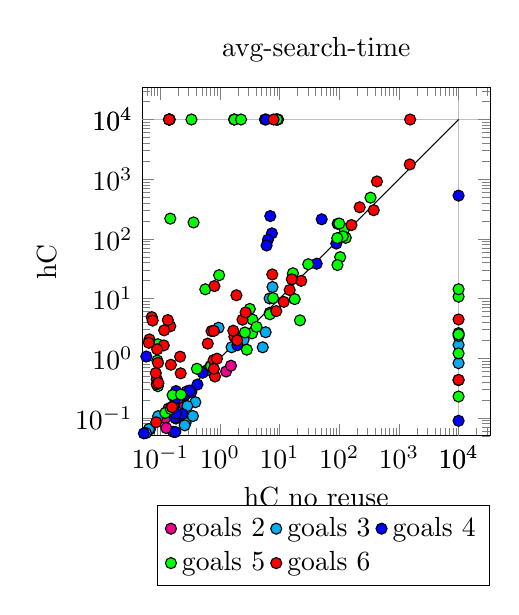
\begin{tikzpicture}
\begin{axis}[extra x tick style={grid=major},
	extra x ticks=10000,
extra y tick style={grid=major},
extra y ticks=10000,
height=6cm,
legend cell align=left,
legend style={at={(1.0,-0.2)}, legend columns=3},
title=avg-search-time,
width=6cm,
xlabel=hC no reuse,
xmin=0.05,
xmode=log,
ylabel=hC,
ymin=0.05,
ymode=log]
\addplot[color=magenta, mark=*, mark options={{draw=black}}, only marks] coordinates {
(0.000337, 0.006320) (0.003333, 0.003333) (0.018661, 0.005222) (0.000349, 0.007541) (0.027055, 0.014731) (0.179249, 0.106756) (0.044858, 0.111396) (0.001134, 0.007828) (0.165205, 0.058350) (0.067012, 0.063801) (0.000345, 0.003490) (0.197661, 0.041971) (0.022867, 0.021803) (0.025771, 0.009210) (0.000671, 0.004323) (0.006874, 0.001146) (0.000311, 0.002643) (0.001131, 0.004955) (0.762613, 0.602015) (0.136985, 0.142653) (0.001338, 0.000775) (0.010000, 0.010000) (0.061649, 0.005312) (0.098613, 0.030961) (0.026615, 0.002005) (0.001360, 0.000498) (0.000744, 0.006762) (0.005791, 0.002067) (0.118864, 0.112418) (0.130353, 0.037755) (0.010938, 0.009739) (0.001055, 0.029812) (0.019191, 0.008746) (0.302018, 0.043711) (0.013194, 0.005753) (0.001445, 0.000433) (0.126939, 0.009533) (0.000342, 0.000532) (0.001410, 0.000651) (0.001023, 0.043706) (0.000314, 0.000716) (0.268536, 0.099624) (0.253824, 0.161702) (0.121452, 0.099550) (0.128185, 0.011167) (0.001117, 0.015114) (0.201670, 0.212821) (0.001429, 0.003878) (0.123754, 0.015713) (0.100055, 0.042183) (0.013980, 0.001141) (0.000342, 0.001008) (0.023366, 0.009129) (0.007072, 0.001941) (0.026508, 0.010474) (0.000667, 0.003102) (0.047128, 0.071080) (0.011319, 0.010497) (0.042066, 0.042300) (0.268836, 0.094522) (0.001455, 0.000421) (0.290460, 0.023557) (0.042038, 0.042319) (1.269460, 0.597827) (0.003333, 0.009926) (0.005996, 0.001176) (0.003333, 0.013868) (0.123515, 0.010629) (0.019653, 0.005564) (0.025268, 0.013444) (0.000327, 0.001677) (0.109958, 0.029603) (0.000323, 0.000607) (0.284140, 0.014276) (0.000329, 0.001424) (0.026181, 0.018984) (0.001429, 0.001429) (0.166027, 0.155805) (0.057937, 0.004638) (0.001512, 0.000389) (10000, 0.015556) (0.205684, 0.020727) (0.006971, 0.001568) (0.000341, 0.002026) (0.001429, 0.005633) (0.020692, 0.005966) (0.126225, 0.067447) (0.007259, 0.001461) (0.013648, 0.001137) (0.131596, 0.021228) (0.276867, 0.276203) (0.001460, 0.001113) (1.533014, 0.747281) (0.013442, 0.003608) (0.018146, 0.004430) (0.025367, 0.009885) (0.059498, 0.003987) (0.000313, 0.000431)
};
\addlegendentry{goals 2}
\addplot[color=cyan, mark=*, mark options={{draw=black}}, only marks] coordinates {
(0.757443, 0.022042) (0.090619, 0.041095) (6.852333, 5.754767) (0.021487, 0.003928) (7.615700, 15.560867) (0.024388, 0.197097) (0.949970, 3.234870) (0.000320, 0.015393) (10000, 0.428058) (0.024167, 0.166367) (0.063648, 0.035249) (0.024121, 0.027799) (6.811400, 10.026000) (0.133464, 0.030088) (0.124401, 0.048315) (0.266267, 0.082843) (0.023613, 0.008806) (0.002715, 0.086262) (0.023848, 0.178984) (0.065611, 0.049612) (0.024209, 0.162352) (10000, 1.672420) (0.001018, 0.032864) (0.000667, 0.022385) (0.023412, 0.014291) (0.000367, 0.032366) (0.256560, 0.074842) (0.353087, 0.107204) (0.001036, 0.047994) (0.000390, 0.033150) (0.001101, 0.044020) (10000, 0.024385) (0.047127, 0.187065) (0.022577, 0.007199) (0.022579, 0.006721) (0.387741, 0.182943) (0.254734, 0.018581) (0.042321, 0.145848) (0.000316, 0.007535) (0.025329, 0.014922) (0.010000, 0.010000) (0.000541, 0.009471) (0.000373, 0.026589) (0.001429, 0.033994) (0.000301, 0.009362) (0.008860, 0.016138) (0.002485, 0.060303) (0.002015, 0.029947) (0.023609, 0.033304) (0.000667, 0.017416) (0.139861, 0.025429) (0.002142, 0.007636) (0.025363, 0.058835) (0.042523, 0.168563) (0.000319, 0.013930) (0.003333, 0.032748) (0.039712, 0.014533) (0.008665, 0.005321) (0.027764, 0.025795) (0.024822, 0.199093) (0.284447, 0.157703) (10000, 2.355102) (0.000573, 0.014172) (0.026769, 0.290407) (0.000323, 0.024716) (5.219556, 1.520497) (0.000372, 0.040962) (0.036466, 0.038221) (0.013571, 0.007934) (0.029081, 0.029566) (0.000380, 0.058324) (0.000381, 0.067176) (1.568700, 1.524820) (0.064637, 0.064888) (0.008602, 0.005871) (0.000620, 0.020287) (2.496350, 2.031780) (0.024219, 0.082145) (0.092336, 0.106600) (0.002647, 0.004190) (10000, 0.034504) (0.582762, 0.618163) (0.003333, 0.020310) (5.836419, 2.720968) (0.008885, 0.003210) (0.022836, 0.038368) (0.041402, 0.037368) (0.012279, 0.019312) (10000, 0.824438) (0.057639, 0.055607) (0.001113, 0.094110) (0.272685, 0.049700) (0.000593, 0.011577) (0.025999, 0.033378) (0.000297, 0.008957) (0.002315, 0.018663) (0.289962, 0.023562) (0.002786, 0.044184)
};
\addlegendentry{goals 3}
\addplot[color=blue, mark=*, mark options={{draw=black}}, only marks] coordinates {
(0.000376, 0.013516) (0.001938, 0.977845) (0.001897, 0.856083) (0.513147, 0.570060) (0.053170, 0.054861) (6.979514, 240.696000) (0.001984, 0.320850) (0.049590, 0.187833) (0.001689, 0.810024) (0.254392, 0.237958) (0.001278, 0.043114) (0.003333, 0.004553) (0.178475, 0.057867) (0.001338, 0.036938) (0.001429, 0.069896) (41.880800, 38.315300) (1.963240, 1.646300) (10000, 0.089129) (0.182998, 0.097368) (0.001626, 0.383037) (0.021844, 0.072184) (0.049266, 0.131422) (0.002217, 0.701371) (0.001264, 0.070159) (0.001395, 0.013913) (0.001830, 0.155188) (0.001482, 0.089123) (0.024042, 0.081130) (89.307300, 83.310200) (0.026276, 10000) (0.001646, 0.161426) (0.001443, 0.015276) (50.762571, 212.608571) (0.001429, 0.067672) (0.012376, 0.014726) (0.001585, 0.266262) (0.002336, 0.894545) (0.001384, 0.034395) (0.183262, 0.280887) (5.684333, 10000) (0.000667, 0.030571) (0.000344, 0.015141) (0.024308, 10000) (0.419938, 0.361739) (0.001710, 0.023645) (0.003126, 0.004231) (0.001820, 2.555840) (7.438533, 123.574444) (0.003333, 0.110117) (0.234768, 0.115825) (0.001465, 0.050085) (0.013246, 0.022897) (94.009000, 178.667333) (0.002270, 0.549024) (5.935756, 10000) (10000, 529.816667) (6.382100, 96.798333) (0.260198, 0.244869) (0.003333, 0.328486) (0.000328, 0.004455) (0.058420, 1.066500) (0.177283, 0.100542) (0.003146, 0.004384) (0.001460, 0.006442) (0.001601, 0.508405) (0.000314, 0.010395) (0.003111, 0.006319) (0.176222, 0.207235) (6.060710, 77.342941) (0.001896, 3.497865) (0.002191, 1.216317) (0.330710, 0.269976) (0.049254, 0.064916) (0.001384, 0.079979) (0.183321, 0.118291) (0.309796, 0.286414) (0.000341, 0.017682) (0.002057, 1.906146) (0.002166, 0.049975) (0.001975, 0.466056) (0.010000, 0.010000) (0.000326, 0.007530) (0.001429, 2.779300) (0.002185, 0.517407) (0.047001, 0.803997)
};
\addlegendentry{goals 4}
\addplot[color=green, mark=*, mark options={{draw=black}}, only marks] coordinates {
(0.003511, 0.310524) (128.628000, 104.126333) (0.022969, 0.023725) (10000, 2.625824) (0.000431, 0.031342) (0.333303, 10000) (3.515907, 4.428120) (0.147329, 218.141000) (3.457290, 2.604732) (0.009024, 0.050187) (30.218400, 37.503700) (0.121296, 0.121056) (2.829747, 1.388687) (0.569895, 14.268683) (0.003333, 0.114103) (17.924677, 9.767645) (0.001429, 6.142157) (6.870990, 5.440640) (121.811571, 148.545714) (0.008051, 10000) (0.091328, 0.339167) (0.003333, 8.566500) (0.091161, 1.711032) (0.008119, 10000) (8.940945, 10000) (0.022825, 0.057943) (9.433452, 10000) (114.788000, 110.049000) (0.007265, 3.896528) (2.626057, 2.695000) (0.002659, 0.145073) (0.003058, 0.429292) (334.567000, 490.006000) (0.089394, 0.912504) (1.726032, 10000) (0.002936, 0.108485) (103.703000, 49.394714) (0.006458, 2.471887) (0.004165, 0.346757) (10000, 10.726693) (0.969865, 24.563000) (10000, 14.307984) (0.000424, 0.015280) (0.003609, 1.027384) (10000, 1.202483) (0.006567, 2.595697) (1.750882, 10000) (0.000470, 0.034337) (0.021895, 0.026280) (0.161172, 0.240178) (0.150109, 0.140528) (0.008503, 10000) (7.765510, 10.157800) (2.260535, 10000) (0.003886, 0.975566) (10000, 0.227517) (0.411680, 0.664280) (0.003492, 28.899533) (92.697333, 102.926000) (8.749097, 10000) (0.007613, 6.785400) (0.003746, 0.807690) (99.983333, 180.416667) (0.002574, 0.055645) (21.959206, 4.300698) (4.110900, 3.342300) (0.361879, 188.261429) (93.324667, 36.410600) (16.752581, 26.472032) (0.692473, 0.733357) (0.711577, 0.735422) (3.170686, 6.685486) (9.014270, 10000) (0.010000, 0.010000) (0.022111, 0.022650) (0.003879, 49.776897) (0.222593, 0.245547) (10000, 2.500134)
};
\addlegendentry{goals 5}
\addplot[color=red, mark=*, mark options={{draw=black}}, only marks] coordinates {
(0.141348, 10000) (0.024145, 1.164115) (0.114505, 1.636932) (0.065925, 2.063243) (0.024557, 1.019929) (7.928952, 10000) (0.140335, 10000) (0.001734, 10000) (0.141435, 10000) (0.085376, 0.084345) (0.072219, 4.869300) (0.088790, 1.407086) (14.752000, 13.856500) (0.725019, 2.842190) (2.389402, 4.411142) (0.826851, 0.492276) (0.001768, 10000) (0.150679, 0.775830) (0.215272, 1.060538) (0.005794, 10000) (0.809590, 16.148903) (7.547548, 25.294742) (428.715000, 916.027000) (0.001978, 6.138333) (0.784217, 0.928031) (0.004291, 7.783698) (0.220103, 0.557403) (0.087518, 0.443344) (10000, 0.432175) (0.003671, 1.361560) (0.006114, 0.314216) (220.006000, 337.925000) (1542.990000, 10000) (1520.650000, 1763.810000) (0.023633, 0.258303) (23.064267, 19.768900) (1.746730, 2.278303) (1.890665, 11.323100) (0.022319, 2.615260) (0.792800, 2.866343) (0.001762, 10000) (0.144599, 10000) (0.064421, 1.809267) (0.084229, 0.562997) (16.043267, 21.050833) (0.793212, 0.662718) (0.003735, 0.687835) (160.223000, 170.076000) (11.734500, 8.785160) (0.625592, 1.753953) (0.021219, 2.879300) (0.147311, 3.423000) (10000, 4.453922) (0.891800, 0.978837) (0.001661, 10000) (0.074712, 4.260329) (1.677429, 2.886629) (8.818960, 6.151750) (0.001946, 0.812283) (0.002699, 10000) (1.945700, 1.989700) (0.087034, 0.365526) (0.140830, 10000) (0.091636, 0.835756) (0.006308, 1.384667) (0.093159, 0.382409) (0.005894, 0.923079) (0.116443, 2.927453) (0.006429, 0.641503) (0.024832, 1.761427) (0.001990, 2.536442) (0.001976, 7.256968) (378.323333, 301.947667) (2.695580, 5.845700) (0.134047, 4.350952) (0.157602, 0.151291)
};
\addlegendentry{goals 6}
\addplot[color=black] coordinates {(0.050000, 0.050000) (10000, 10000)};
\end{axis}
\end{tikzpicture}

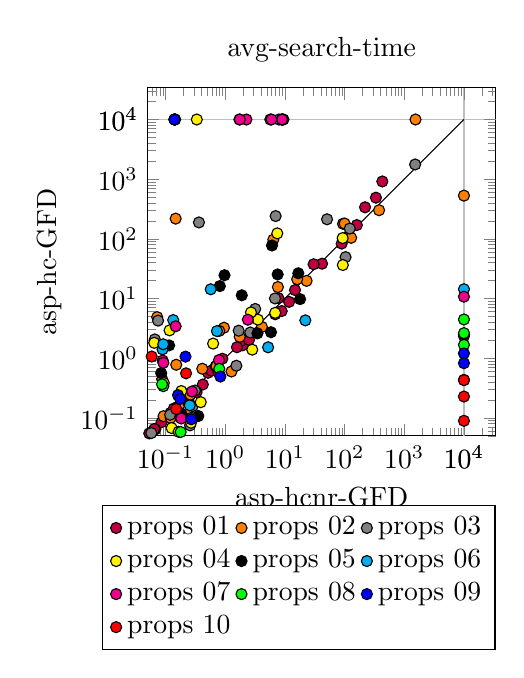
\begin{tikzpicture}
\begin{axis}[extra x tick style={grid=major},
	extra x ticks=10000,
extra y tick style={grid=major},
extra y ticks=10000,
height=6cm,
legend cell align=left,
legend style={at={(1,-0.2)}, legend columns=3},
title=avg-search-time,
width=6cm,
xlabel=asp-hcnr-GFD,
xmin=0.05,
xmode=log,
ylabel=asp-hc-GFD,
ymin=0.05,
ymode=log]
\addplot[color=purple, mark=*, mark options={{draw=black}}, only marks] coordinates {
(0.513147, 0.570060) (0.053170, 0.054861) (114.788000, 110.049000) (0.029081, 0.029566) (0.085376, 0.084345) (41.880800, 38.315300) (1.963240, 1.646300) (0.121296, 0.121056) (6.870990, 5.440640) (0.582762, 0.618163) (428.715000, 916.027000) (8.818960, 6.151750) (0.419938, 0.361739) (0.011319, 0.010497) (220.006000, 337.925000) (0.042066, 0.042300) (89.307300, 83.310200) (7.765510, 10.157800) (334.567000, 490.006000) (0.067012, 0.063801) (0.042038, 0.042319) (160.223000, 170.076000) (11.734500, 8.785160) (0.022867, 0.021803) (0.041402, 0.037368) (0.254392, 0.237958) (0.891800, 0.978837) (0.762613, 0.602015) (0.036466, 0.038221) (0.330710, 0.269976) (1.945700, 1.989700) (0.012376, 0.014726) (0.136985, 0.142653) (1.568700, 1.524820) (0.201670, 0.212821) (0.692473, 0.733357) (0.064637, 0.064888) (0.222593, 0.245547) (0.010000, 0.010000) (14.752000, 13.856500) (2.496350, 2.031780) (0.157602, 0.151291) (30.218400, 37.503700)
};
\addlegendentry{props 01}
\addplot[color=orange, mark=*, mark options={{draw=black}}, only marks] coordinates {
(128.628000, 104.126333) (0.166027, 0.155805) (0.049590, 0.187833) (0.147329, 218.141000) (0.003333, 0.032748) (0.023366, 0.009129) (0.072219, 4.869300) (0.092336, 0.106600) (0.949970, 3.234870) (0.027764, 0.025795) (0.003333, 0.114103) (1542.990000, 10000) (0.090619, 0.041095) (0.234768, 0.115825) (0.003333, 0.110117) (0.003333, 8.566500) (0.063648, 0.035249) (0.010938, 0.009739) (0.003333, 0.004553) (23.064267, 19.768900) (1.746730, 2.278303) (0.792800, 2.866343) (0.022319, 2.615260) (1.269460, 0.597827) (0.003333, 0.009926) (16.043267, 21.050833) (0.150679, 0.775830) (10000, 529.816667) (6.382100, 96.798333) (0.260198, 0.244869) (0.003333, 0.328486) (0.003333, 0.013868) (0.065611, 0.049612) (0.121452, 0.099550) (0.411680, 0.664280) (94.009000, 178.667333) (99.983333, 180.416667) (7.615700, 15.560867) (4.110900, 3.342300) (0.711577, 0.735422) (0.003333, 0.020310) (0.042523, 0.168563) (0.010000, 0.010000) (378.323333, 301.947667) (0.003333, 0.003333) (0.100055, 0.042183) (0.047001, 0.803997)
};
\addlegendentry{props 02}
\addplot[color=gray, mark=*, mark options={{draw=black}}, only marks] coordinates {
(0.003511, 0.310524) (6.979514, 240.696000) (0.001429, 0.001429) (0.065925, 2.063243) (0.001429, 0.069896) (0.124401, 0.048315) (0.005791, 0.002067) (121.811571, 148.545714) (0.256560, 0.074842) (0.049266, 0.131422) (0.118864, 0.112418) (0.001429, 6.142157) (0.179249, 0.106756) (0.087518, 0.443344) (0.284447, 0.157703) (0.001626, 0.383037) (50.762571, 212.608571) (0.001429, 0.067672) (6.811400, 10.026000) (0.001465, 0.050085) (1520.650000, 1763.810000) (2.626057, 2.695000) (0.019191, 0.008746) (0.013194, 0.005753) (0.042321, 0.145848) (0.098613, 0.030961) (0.001429, 0.005633) (0.026769, 0.290407) (1.533014, 0.747281) (0.021219, 2.879300) (0.002715, 0.086262) (0.001429, 0.033994) (0.002485, 0.060303) (0.001946, 0.812283) (0.074712, 4.260329) (1.677429, 2.886629) (0.057639, 0.055607) (0.002659, 0.145073) (0.361879, 188.261429) (3.170686, 6.685486) (0.309796, 0.286414) (103.703000, 49.394714) (0.001429, 0.003878) (0.001429, 2.779300)
};
\addlegendentry{props 03}
\addplot[color=yellow, mark=*, mark options={{draw=black}}, only marks] coordinates {
(0.001820, 2.555840) (0.000667, 0.022385) (0.333303, 10000) (3.515907, 4.428120) (0.001338, 0.036938) (2.829747, 1.388687) (0.000667, 0.003102) (0.001978, 6.138333) (0.003671, 1.361560) (0.020692, 0.005966) (0.044858, 0.111396) (0.126225, 0.067447) (0.183262, 0.280887) (0.000667, 0.030571) (0.165205, 0.058350) (0.387741, 0.182943) (0.006458, 2.471887) (0.064421, 1.809267) (0.266267, 0.082843) (0.001460, 0.001113) (0.625592, 1.753953) (0.005996, 0.001176) (0.000671, 0.004323) (6.852333, 5.754767) (0.001601, 0.508405) (0.024209, 0.162352) (0.013442, 0.003608) (0.002015, 0.029947) (0.003492, 28.899533) (92.697333, 102.926000) (0.000667, 0.017416) (0.049254, 0.064916) (0.001384, 0.079979) (0.025367, 0.009885) (93.324667, 36.410600) (0.093159, 0.382409) (0.002936, 0.108485) (0.116443, 2.927453) (7.438533, 123.574444) (0.024219, 0.082145) (2.695580, 5.845700) (0.133464, 0.030088) (0.002786, 0.044184)
};
\addlegendentry{props 04}
\addplot[color=black, mark=*, mark options={{draw=black}}, only marks] coordinates {
(0.000376, 0.013516) (0.001938, 0.977845) (0.114505, 1.636932) (0.001264, 0.070159) (0.000342, 0.001008) (0.272685, 0.049700) (0.003735, 0.687835) (0.141435, 10000) (0.018661, 0.005222) (3.457290, 2.604732) (0.000744, 0.006762) (0.002647, 0.004190) (0.353087, 0.107204) (0.809590, 16.148903) (17.924677, 9.767645) (0.006567, 2.595697) (0.047128, 0.071080) (0.001482, 0.089123) (0.130353, 0.037755) (9.433452, 10000) (0.001990, 2.536442) (1.890665, 11.323100) (7.547548, 25.294742) (5.836419, 2.720968) (0.969865, 24.563000) (0.084229, 0.562997) (0.013246, 0.022897) (0.000323, 0.024716) (0.197661, 0.041971) (0.023848, 0.178984) (0.183321, 0.118291) (0.025771, 0.009210) (0.000381, 0.067176) (6.060710, 77.342941) (8.749097, 10000) (0.002191, 1.216317) (0.002574, 0.055645) (0.000327, 0.001677) (0.139861, 0.025429) (16.752581, 26.472032) (0.007259, 0.001461) (0.001338, 0.000775) (0.025999, 0.033378) (0.002315, 0.018663) (0.003879, 49.776897)
};
\addlegendentry{props 05}
\addplot[color=cyan, mark=*, mark options={{draw=black}}, only marks] coordinates {
(0.088790, 1.407086) (0.001278, 0.043114) (0.024388, 0.197097) (0.039712, 0.014533) (0.000326, 0.007530) (0.000349, 0.007541) (0.205684, 0.020727) (0.569895, 14.268683) (0.005794, 10000) (0.004291, 7.783698) (0.007613, 6.785400) (0.091161, 1.711032) (0.134047, 4.350952) (0.001585, 0.266262) (1.726032, 10000) (10000, 14.307984) (0.131596, 0.021228) (0.003609, 1.027384) (0.144599, 10000) (0.002270, 0.549024) (5.219556, 1.520497) (0.001410, 0.000651) (0.001023, 0.043706) (0.253824, 0.161702) (0.177283, 0.100542) (0.007072, 0.001941) (0.725019, 2.842190) (0.008860, 0.016138) (0.000380, 0.058324) (0.024042, 0.081130) (5.684333, 10000) (0.018146, 0.004430) (0.001897, 0.856083) (7.928952, 10000) (0.009024, 0.050187) (0.002142, 0.007636) (0.025363, 0.058835) (0.024121, 0.027799) (0.000323, 0.000607) (9.014270, 10000) (0.000301, 0.009362) (0.001976, 7.256968) (0.289962, 0.023562) (21.959206, 4.300698) (0.026181, 0.018984)
};
\addlegendentry{props 06}
\addplot[color=magenta, mark=*, mark options={{draw=black}}, only marks] coordinates {
(0.000337, 0.006320) (0.027055, 0.014731) (0.000328, 0.004455) (0.001689, 0.810024) (10000, 10.726693) (2.260535, 10000) (0.001360, 0.000498) (0.000329, 0.001424) (2.389402, 4.411142) (0.182998, 0.097368) (0.006971, 0.001568) (0.021844, 0.072184) (0.002217, 0.701371) (0.089394, 0.912504) (0.784217, 0.928031) (0.001101, 0.044020) (8.940945, 10000) (0.001055, 0.029812) (0.024557, 1.019929) (0.007265, 3.896528) (10000, 2.355102) (0.302018, 0.043711) (0.254734, 0.018581) (0.000367, 0.032366) (0.276867, 0.276203) (0.000541, 0.009471) (1.750882, 10000) (0.022836, 0.038368) (5.935756, 10000) (0.147311, 3.423000) (0.123754, 0.015713) (0.141348, 10000) (0.013571, 0.007934) (0.001661, 10000) (0.019653, 0.005564) (0.023609, 0.033304) (0.004165, 0.346757) (0.091636, 0.835756) (0.005894, 0.923079) (0.000297, 0.008957) (0.001975, 0.466056) (0.022111, 0.022650) (0.001384, 0.034395) (0.008665, 0.005321) (10000, 2.500134)
};
\addlegendentry{props 07}
\addplot[color=green, mark=*, mark options={{draw=black}}, only marks] coordinates {
(0.757443, 0.022042) (0.268536, 0.099624) (10000, 2.625824) (0.000431, 0.031342) (0.023412, 0.014291) (0.000316, 0.007535) (0.178475, 0.057867) (0.003146, 0.004384) (0.001768, 10000) (0.001036, 0.047994) (0.001830, 0.155188) (0.008051, 10000) (0.091328, 0.339167) (0.024167, 0.166367) (0.001443, 0.015276) (0.022577, 0.007199) (0.002336, 0.894545) (0.140830, 10000) (0.793212, 0.662718) (0.000344, 0.015141) (0.000573, 0.014172) (0.001445, 0.000433) (0.000373, 0.026589) (10000, 4.453922) (0.021895, 0.026280) (0.000314, 0.000716) (0.059498, 0.003987) (0.123515, 0.010629) (0.006874, 0.001146) (0.000311, 0.002643) (0.026276, 10000) (0.001896, 3.497865) (0.003746, 0.807690) (0.087034, 0.365526) (0.001117, 0.015114) (0.006308, 1.384667) (0.025268, 0.013444) (0.024832, 1.761427) (10000, 1.672420) (0.284140, 0.014276) (0.008602, 0.005871)
};
\addlegendentry{props 08}
\addplot[color=blue, mark=*, mark options={{draw=black}}, only marks] coordinates {
(0.024145, 1.164115) (0.001018, 0.032864) (0.013980, 0.001141) (0.140335, 10000) (0.000314, 0.010395) (0.021487, 0.003928) (0.026508, 0.010474) (0.001734, 10000) (0.826851, 0.492276) (0.215272, 1.060538) (10000, 0.034504) (0.001395, 0.013913) (0.000424, 0.015280) (0.024822, 0.199093) (0.022825, 0.057943) (0.268836, 0.094522) (0.001455, 0.000421) (0.290460, 0.023557) (0.024308, 10000) (0.126939, 0.009533) (0.008885, 0.003210) (0.000320, 0.015393) (0.000345, 0.003490) (10000, 1.202483) (0.025329, 0.014922) (0.000372, 0.040962) (0.000342, 0.000532) (0.161172, 0.240178) (0.003886, 0.975566) (0.003111, 0.006319) (0.001131, 0.004955) (0.176222, 0.207235) (0.008503, 10000) (10000, 0.824438) (0.000593, 0.011577) (0.002057, 1.906146) (0.001646, 0.161426) (0.061649, 0.005312) (0.002185, 0.517407) (0.006429, 0.641503)
};
\addlegendentry{props 09}
\addplot[color=red, mark=*, mark options={{draw=black}}, only marks] coordinates {
(0.000319, 0.013930) (0.047127, 0.187065) (0.057937, 0.004638) (0.000341, 0.017682) (0.000470, 0.034337) (0.001512, 0.000389) (10000, 0.015556) (0.026615, 0.002005) (0.150109, 0.140528) (10000, 0.089129) (0.013648, 0.001137) (0.000341, 0.002026) (0.002166, 0.049975) (0.000390, 0.033150) (10000, 0.024385) (10000, 0.432175) (0.008119, 10000) (0.006114, 0.314216) (0.001460, 0.006442) (0.022579, 0.006721) (0.023633, 0.258303) (0.001134, 0.007828) (0.003058, 0.429292) (0.001710, 0.023645) (0.003126, 0.004231) (0.023613, 0.008806) (0.058420, 1.066500) (0.012279, 0.019312) (10000, 0.227517) (10000, 0.428058) (0.001762, 10000) (0.002699, 10000) (0.128185, 0.011167) (0.001113, 0.094110) (0.109958, 0.029603) (0.001984, 0.320850) (0.220103, 0.557403) (0.022969, 0.023725) (0.000620, 0.020287) (0.000313, 0.000431)
};
\addlegendentry{props 10}
\addplot[color=black] coordinates {(0.050000, 0.050000) (10000, 10000)};
\end{axis}
\end{tikzpicture}

\caption{Comparison average earch time per meta node per task in nomystery. hC: propagates the learned heuristic down the meta search tree, hC no reuse: computes the heuristic for every meta search node from scratch}
\end{figure}

%\newpage
%\begin{figure}[ht]
%\input{data/action_set_properties/scatterplot-expansions_C-Cnr_tpp_goals.tex}
%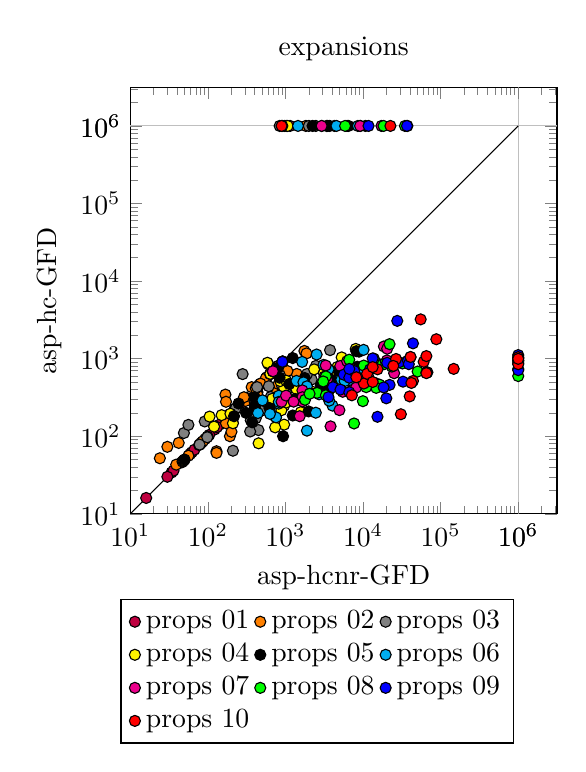
\begin{tikzpicture}
\begin{axis}[extra x tick style={grid=major}, extra x ticks=1000000, 
		extra y tick style={grid=major}, extra y ticks=1000000, height=7cm, 
		legend cell align=left, legend style={at={(0.9, -0.2)}, legend columns=3}, 
		title=expansions, width=7cm, xlabel=asp-hcnr-GFD, xmin=10, xmode=log, 
		ylabel=asp-hc-GFD, ymin=10, ymode=log]
\addplot[color=purple, mark=*, mark options={{draw=black}}, only marks] coordinates {
(220, 220) (85, 85) (122, 122) (428, 428) (313, 313) (631, 631) (16, 16) (92, 92) (141, 141) (59, 59) (46, 46) (570, 570) (1146, 1000000) (168, 168) (285, 285) (62, 62) (104, 104) (79, 79) (192, 192) (577, 577) (50, 50) (455, 455) (99, 99) (67, 67) (973, 1000000) (475, 475) (34, 34) (271, 271) (757, 757) (131, 131) (221, 221) (758, 758) (36, 36) (183, 183) (305, 305) (8, 8) (30, 30) (711, 711)
};
\addlegendentry{props 01}
\addplot[color=orange, mark=*, mark options={{draw=black}}, only marks] coordinates {
(1752, 1257) (168, 344) (77, 77) (207, 153) (184, 184) (435, 369) (366, 429) (42, 82) (306, 285) (56, 56) (855, 607) (192, 100) (129, 64) (435, 341) (1398, 635) (201, 114) (414, 262) (171, 147) (24, 52) (759, 403) (1000000, 735) (556, 556) (82, 82) (812, 812) (171, 278) (291, 318) (39, 43) (227, 227) (813, 470) (1863, 1167) (86, 86) (30, 73) (476, 476) (1059, 692) (632, 632) (414, 414) (129, 61) (47, 47) (1824, 1000000)
};
\addlegendentry{props 02}
\addplot[color=gray, mark=*, mark options={{draw=black}}, only marks] coordinates {
(2177, 539) (448, 120) (1995, 1000000) (735, 180) (840, 1000000) (350, 115) (3717, 1000000) (210, 65) (609, 441) (966, 294) (2933, 1000000) (636, 636) (434, 251) (2457, 1000000) (357, 160) (78, 78) (49, 110) (399, 279) (1421, 481) (48, 48) (413, 170) (483, 212) (399, 223) (98, 97) (847, 614) (2401, 742) (91, 155) (1015, 371) (1897, 635) (56, 140) (2471, 808) (228, 228) (280, 632) (3752, 1287) (430, 430) (1027, 1000000) (903, 445) (644, 321)
};
\addlegendentry{props 03}
\addplot[color=yellow, mark=*, mark options={{draw=black}}, only marks] coordinates {
(960, 417) (960, 248) (120, 133) (1065, 1000000) (4665, 781) (2340, 727) (885, 216) (4275, 1000000) (637, 637) (1020, 272) (960, 141) (2160, 379) (735, 130) (105, 179) (49, 49) (600, 851) (8040, 1335) (150, 187) (585, 885) (210, 147) (450, 81) (195, 195) (3120, 651) (645, 247) (6210, 1000000) (3390, 1000000) (1575, 204) (1380, 407) (855, 514) (1020, 520) (2070, 361) (4065, 679) (675, 304) (5295, 1038)
};
\addlegendentry{props 04}
\addplot[color=black, mark=*, mark options={{draw=black}}, only marks] coordinates {
(1333, 302) (806, 769) (1240, 185) (4836, 694) (1798, 365) (403, 245) (8401, 786) (2232, 1000000) (10726, 1000000) (1116, 471) (1984, 209) (1767, 563) (50, 50) (3348, 494) (372, 151) (2852, 454) (620, 231) (1240, 1017) (403, 313) (310, 200) (8866, 1231) (8184, 1248) (3503, 1000000) (248, 264) (3627, 388) (919, 919) (837, 568) (930, 100) (6479, 1000000) (3906, 534) (686, 686) (217, 181) (403, 235)
};
\addlegendentry{props 05}
\addplot[color=cyan, mark=*, mark options={{draw=black}}, only marks] coordinates {
(7371, 464) (917, 917) (5229, 537) (4032, 248) (1449, 1000000) (9828, 752) (7938, 579) (10143, 1298) (4536, 1000000) (3654, 287) (441, 199) (819, 333) (1638, 908) (756, 175) (2457, 201) (1386, 517) (630, 194) (17073, 841) (819, 263) (3591, 729) (1701, 495) (504, 290) (1890, 440) (5796, 513) (2520, 1131) (819, 277) (9198, 1000000) (8568, 1000000) (2709, 347) (3087, 831) (1890, 118) (687, 687)
};
\addlegendentry{props 06}
\addplot[color=magenta, mark=*, mark options={{draw=black}}, only marks] coordinates {
(5461, 374) (1651, 281) (25146, 649) (3429, 534) (14859, 477) (889, 278) (10541, 565) (18542, 1436) (3810, 134) (20320, 949) (1651, 390) (9144, 1000000) (5080, 804) (20447, 1343) (11684, 584) (1651, 318) (688, 688) (7239, 736) (6223, 928) (4953, 217) (2921, 1000000) (1016, 334) (3175, 586) (1000000, 934) (7366, 398) (1270, 279) (918, 918) (1524, 181) (17272, 1000000) (16002, 801) (8128, 424) (3302, 816)
};
\addlegendentry{props 07}
\addplot[color=green, mark=*, mark options={{draw=black}}, only marks] coordinates {
(910, 1000000) (18870, 852) (16320, 462) (1000000, 596) (14535, 861) (21930, 1538) (6630, 969) (18360, 1000000) (6885, 615) (23460, 790) (50490, 682) (2550, 362) (6120, 610) (14790, 420) (13770, 999) (40800, 1044) (3315, 590) (1785, 295) (10200, 814) (9945, 283) (5865, 1000000) (2040, 352) (37230, 1000000) (34680, 1000000) (3315, 337) (3060, 508) (32130, 867) (10965, 429) (7650, 146)
};
\addlegendentry{props 08}
\addplot[color=blue, mark=*, mark options={{draw=black}}, only marks] coordinates {
(5621, 622) (67452, 667) (15330, 178) (12264, 726) (43946, 1574) (6643, 568) (4088, 429) (19929, 308) (20440, 883) (29127, 896) (36792, 1000000) (32704, 505) (3577, 319) (5110, 399) (37814, 942) (13286, 1008) (6643, 369) (11753, 1000000) (7665, 694) (21973, 459) (1000000, 711) (1000000, 1112) (1000000, 949) (1000000, 1021) (18396, 426) (911, 911) (6643, 737) (38836, 849) (27594, 3068)
};
\addlegendentry{props 09}
\addplot[color=red, mark=*, mark options={{draw=black}}, only marks] coordinates {
(7161, 337) (87978, 1779) (30690, 192) (43989, 516) (1000000, 877) (65472, 663) (10230, 478) (60357, 910) (8184, 575) (1000000, 1045) (15345, 729) (1000000, 848) (147312, 738) (11253, 638) (65472, 650) (41943, 486) (13299, 500) (55242, 3208) (1000000, 994) (40920, 1051) (13299, 779) (39897, 326) (26598, 990) (889, 1000000) (24552, 806) (22506, 1000000) (65472, 1079)
};
\addlegendentry{props 10}
\addplot[color=black] coordinates {(0.050000, 0.050000) (1000000, 1000000)};
\end{axis}
\end{tikzpicture}

%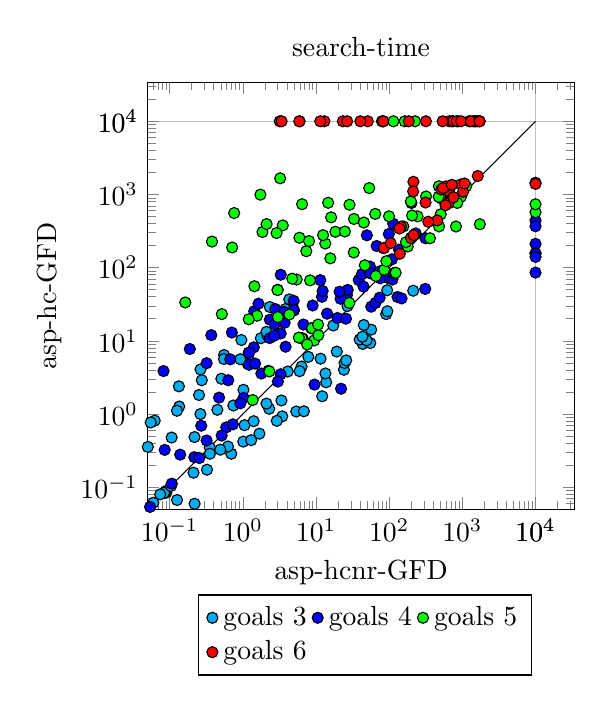
\begin{tikzpicture}
\begin{axis}[extra x tick style={grid=major}, extra x ticks=10000, 
	extra y tick style={grid=major}, extra y ticks=10000, height=7cm, 
	legend cell align=left, legend style={at={(0.9, -0.2)}, legend columns=3}, 
	title=search-time, width=7cm, xlabel=asp-hcnr-GFD, xmin=0.05, xmode=log, ylabel=asp-hc-GFD, ymin=0.05, ymode=log]
\addplot[color=cyan, mark=*, mark options={{draw=black}}, only marks] coordinates {
(0.012686, 0.018468) (13.777100, 2.710320) (19.240200, 7.120620) (0.090099, 0.083997) (2.235020, 3.897000) (0.218968, 0.059241) (43.474200, 9.070310) (5.364710, 1.079980) (0.051041, 0.048613) (2.290610, 1.176320) (0.741274, 1.304950) (24.066500, 4.017910) (1.055250, 0.702632) (6.354300, 4.442340) (90.877300, 23.160200) (93.913600, 49.026600) (0.047240, 0.032462) (0.263980, 4.060410) (0.087937, 0.087912) (1.684110, 0.537619) (1.758720, 10.837800) (0.010000, 0.010000) (0.323599, 0.172992) (0.694918, 0.286133) (0.011962, 0.196532) (0.625814, 0.359063) (0.109042, 0.049356) (4.109860, 3.801110) (2.334540, 28.923300) (213.176000, 48.347800) (39.496600, 10.410300) (26.936400, 29.782600) (1.013270, 0.418749) (3.455810, 0.927333) (0.059770, 0.061135) (1.168960, 6.025890) (6.826830, 1.087410) (0.553401, 6.379160) (0.353499, 0.348109) (1.169700, 4.838980) (0.263053, 0.997536) (0.028932, 0.029786) (5.971980, 3.843950) (2.167970, 11.815100) (2.911860, 0.805406) (0.026584, 0.027641) (0.211461, 0.157457) (0.448392, 1.140220) (24.607800, 4.980320) (1.298650, 0.438021) (55.213600, 9.320400) (0.218497, 0.482936) (0.010861, 0.011967) (0.039108, 0.038952) (49.164400, 10.147900) (94.361600, 25.345400) (56.719400, 14.195200) (4.313840, 36.791700) (0.274739, 2.889950) (1.019290, 2.138070) (0.106340, 0.475902) (0.024822, 0.028767) (0.012186, 0.010000) (0.134875, 1.261720) (0.133598, 2.382330) (0.126099, 0.066667) (0.027139, 0.026656) (0.029112, 0.745081) (17.217100, 16.190800) (3.814990, 27.108400) (0.062388, 0.809774) (2.102800, 1.384390) (3.366070, 1.527520) (44.927300, 16.432900) (0.054971, 0.763861) (0.083944, 0.083588) (12.149900, 1.744320) (25.847500, 5.399750) (0.954348, 10.254100) (0.031984, 0.967532) (11.546400, 5.693150) (0.041545, 0.043900) (0.508750, 3.028120) (0.011869, 0.012096) (0.552349, 5.633040) (1.405690, 0.795521) (0.492758, 0.325301) (13.434200, 3.575160) (0.922851, 5.591520) (0.104341, 0.103738) (0.125756, 1.105880) (0.028317, 0.028907) (7.848800, 6.027390) (43.094800, 11.387100) (0.010043, 0.108707) (0.050231, 0.354371) (0.252034, 1.813100) (0.354536, 0.285740) (2.103460, 13.249500) (0.074183, 0.079645)
};
\addlegendentry{goals 3}
\addplot[color=blue, mark=*, mark options={{draw=black}}, only marks] coordinates {
(0.593416, 0.655578) (4.991990, 25.909400) (94.670600, 72.712200) (0.708234, 12.965200) (10000, 439.668000) (111.087000, 68.821400) (3.286660, 12.576600) (38.302300, 67.667400) (0.217147, 0.256366) (24.351700, 40.338200) (136.530000, 175.756000) (0.188454, 7.713660) (0.106920, 0.111535) (10000, 85.518600) (14.161500, 23.475500) (230.472000, 293.598000) (1.431430, 25.373300) (0.020963, 1.130940) (0.254451, 0.249715) (0.043534, 0.125005) (0.730083, 0.721303) (12.048000, 39.922500) (2.336390, 19.454400) (0.671829, 5.578140) (1.635800, 32.079800) (54.536700, 103.330000) (10000, 211.323000) (19.628600, 20.478900) (0.320074, 4.939490) (3.840790, 8.301850) (49.498200, 276.354000) (21.986800, 2.212290) (2.331500, 10.879500) (9.540610, 2.516980) (313.156000, 251.765000) (2.779630, 27.132800) (0.473147, 1.672130) (56.836500, 29.249000) (0.010000, 0.010000) (26.462800, 42.109600) (0.319681, 0.433884) (0.010000, 0.099429) (64.978900, 32.843100) (4.947870, 35.195900) (3.293050, 79.948600) (1.410290, 8.130530) (115.646000, 84.004400) (10000, 157.252000) (8.620140, 14.828600) (10000, 155.684000) (130.014000, 39.685500) (3.657250, 24.808200) (42.461900, 81.394200) (1.790710, 3.568160) (1.215490, 4.708270) (1.202190, 6.895400) (75.287900, 71.494200) (0.270100, 0.690682) (6.733820, 16.688000) (10000, 140.195000) (74.105300, 38.812500) (27.131800, 49.541900) (113.485000, 397.455000) (12.313300, 47.950600) (75.186800, 89.215700) (98.904900, 288.281000) (1.217140, 6.863820) (310.755000, 51.155700) (0.513277, 0.506373) (0.053864, 0.053605) (147.762000, 37.935500) (0.632161, 2.886310) (55.128500, 83.671800) (21.661800, 37.521400) (21.004000, 46.895400) (108.923000, 129.789000) (3.720920, 17.624200) (6.588940, 10.738000) (3.281640, 3.489010) (10000, 367.569000) (0.018648, 0.119977) (0.370328, 11.936300) (0.139223, 0.277867) (2.685970, 11.736100) (0.082363, 3.856860) (2.720190, 16.847800) (1.022730, 1.658470) (3.008850, 2.767970) (0.085493, 0.322556) (11.453000, 67.369300) (67.396500, 197.516000) (8.995970, 30.391500) (0.044703, 1.426120) (0.923861, 1.397460) (83.595100, 184.298000) (44.591600, 54.930500) (25.673600, 20.051800) (4.948640, 26.655400) (201.609000, 763.914000) (1.471410, 4.876470)
};
\addlegendentry{goals 4}
\addplot[color=green, mark=*, mark options={{draw=black}}, only marks] coordinates {
(65.699500, 76.973500) (33.029700, 462.106000) (1.852760, 306.413000) (85.545600, 93.564900) (710.068000, 10000) (10000, 571.317000) (0.713880, 188.591000) (512.504000, 879.127000) (8.294470, 66.970100) (13.385700, 213.494000) (4.316110, 22.851000) (45.032200, 413.287000) (83.375100, 10000) (360.932000, 251.963000) (18.393700, 308.729000) (10000, 734.552000) (1735.270000, 391.493000) (3.010810, 21.065000) (9.445270, 10.116500) (12.485100, 277.765000) (179.289000, 194.451000) (5.439540, 68.688500) (163.069000, 10000) (0.163415, 33.392300) (0.761220, 556.889000) (16.085900, 486.712000) (197.937000, 802.118000) (28.660700, 723.484000) (0.378776, 226.852000) (1414.390000, 10000) (3.509460, 377.575000) (7.364590, 167.650000) (91.394800, 122.391000) (8.840550, 14.874200) (14.642700, 769.436000) (32.797700, 160.973000) (6.374390, 10.832400) (28.544300, 32.917700) (1.562870, 21.993700) (1.204740, 19.694200) (10.772200, 11.929500) (506.075000, 535.652000) (225.421000, 10000) (2.989640, 49.866800) (1.437750, 55.656500) (122.575000, 85.186200) (477.826000, 1293.500000) (169.694000, 222.926000) (2.889180, 296.792000) (1130.330000, 1300.800000) (818.041000, 364.843000) (956.134000, 928.888000) (1.737950, 992.840000) (5.931930, 256.310000) (8.019290, 230.953000) (480.645000, 365.696000) (99.482500, 502.377000) (10000, 1446.680000) (852.304000, 766.589000) (15.696900, 133.887000) (6.452530, 735.922000) (0.516290, 23.136000) (319.536000, 939.201000) (7.574030, 8.905050) (46.415000, 107.579000) (474.571000, 927.586000) (4.733110, 70.585300) (24.803800, 311.645000) (3.235740, 1660.440000) (244.168000, 501.494000) (2.299860, 3.816750) (114.088000, 10000) (2.981500, 49.288800) (5.825620, 11.045300) (10.680400, 16.646200) (205.580000, 515.996000) (53.353900, 1221.450000) (156.032000, 365.378000) (64.458200, 542.436000) (1.364070, 1.549990) (2.111470, 393.522000)
};
\addlegendentry{goals 5}
\addplot[color=red, mark=*, mark options={{draw=black}}, only marks] coordinates {
(13.033600, 10000) (185.057000, 10000) (197.682000, 254.174000) (23.245500, 10000) (879.000000, 10000) (630.051000, 786.688000) (662.202000, 10000) (50.998800, 10000) (748.435000, 10000) (5.962050, 10000) (1492.600000, 10000) (3.196190, 10000) (453.890000, 441.892000) (79.578700, 10000) (3.381850, 10000) (215.517000, 277.873000) (85.088300, 185.556000) (26.615600, 10000) (1723.770000, 10000) (314.205000, 775.662000) (1240.110000, 10000) (317.620000, 10000) (956.424000, 1372.160000) (145.371000, 363.671000) (137.854000, 342.459000) (1024.040000, 1087.160000) (139.634000, 154.579000) (342.210000, 423.418000) (1604.330000, 10000) (10000, 1395.500000) (104.695000, 215.797000) (834.167000, 10000) (214.339000, 1489.210000) (40.341700, 10000) (956.087000, 10000) (514.427000, 1167.470000) (659.598000, 1103.580000) (649.701000, 758.802000) (596.676000, 1286.690000) (544.156000, 1223.120000) (537.926000, 10000) (1517.460000, 10000) (1626.110000, 1786.550000) (82.827300, 10000) (212.711000, 1098.330000) (5.911980, 10000) (588.183000, 712.668000) (11.427400, 10000) (1306.220000, 10000) (718.448000, 1353.800000) (754.553000, 914.113000) (1718.960000, 10000) (1068.970000, 1410.650000)
};
\addlegendentry{goals 6}
\addplot[color=black] coordinates {(0.050000, 0.050000) (10000, 10000)};
\end{axis}
\end{tikzpicture}

%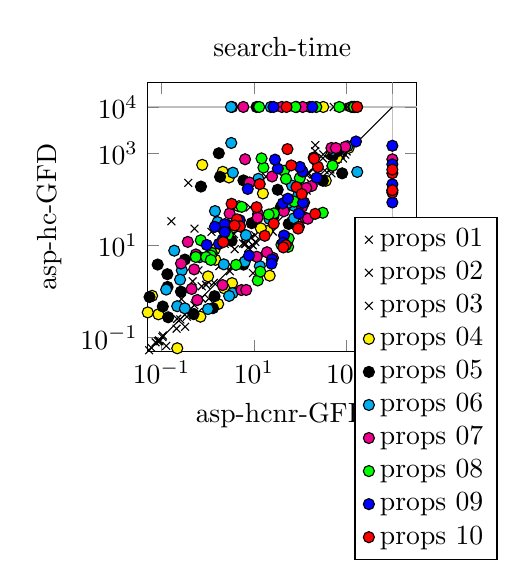
\begin{tikzpicture}
\begin{axis}[extra x tick style={grid=major}, extra x ticks=10000, extra y tick style={grid=major}, extra y ticks=10000, height=5cm, legend cell align=left, legend style={at={(1.3, 0.5)}}, title=search-time, width=5cm, xlabel=asp-hcnr-GFD, xmin=0.05, xmode=log, ylabel=asp-hc-GFD, ymin=0.05, ymode=log]
\addplot[color=blue, mark=x, mark options={{draw=black}}, only marks] coordinates {
(65.699500, 76.973500) (3.281640, 3.489010) (85.545600, 93.564900) (197.682000, 254.174000) (215.517000, 277.873000) (1.790710, 3.568160) (0.090099, 0.083997) (0.010861, 0.011967) (137.854000, 342.459000) (453.890000, 441.892000) (1604.330000, 10000) (0.217147, 0.256366) (9.445270, 10.116500) (1.022730, 1.658470) (0.011869, 0.012096) (0.051041, 0.048613) (8.840550, 14.874200) (0.059770, 0.061135) (28.544300, 32.917700) (0.106920, 0.111535) (139.634000, 154.579000) (0.039108, 0.038952) (0.513277, 0.506373) (0.053864, 0.053605) (956.087000, 10000) (0.012186, 0.010000) (0.923861, 1.397460) (7.574030, 8.905050) (0.730083, 0.721303) (1024.040000, 1087.160000) (0.027139, 0.026656) (2.299860, 3.816750) (588.183000, 712.668000) (5.825620, 11.045300) (10.680400, 16.646200) (718.448000, 1353.800000) (0.010000, 0.010000) (1.364070, 1.549990) (0.074183, 0.079645)
};
\addlegendentry{props 01}
\addplot[color=red, mark=x, mark options={{draw=black}}, only marks] coordinates {
(3.720920, 17.624200) (0.012686, 0.018468) (0.018648, 0.119977) (314.205000, 775.662000) (480.645000, 365.696000) (3.840790, 8.301850) (2.685970, 11.736100) (3.010810, 21.065000) (748.435000, 10000) (0.163415, 33.392300) (10.772200, 11.929500) (0.041545, 0.043900) (25.673600, 20.051800) (85.088300, 185.556000) (0.270100, 0.690682) (10000, 1395.500000) (145.371000, 363.671000) (3.008850, 2.767970) (0.473147, 1.672130) (1.562870, 21.993700) (0.516290, 23.136000) (8.294470, 66.970100) (342.210000, 423.418000) (0.353499, 0.348109) (0.104341, 0.103738) (214.339000, 1489.210000) (0.254451, 0.249715) (0.010000, 0.099429) (0.047240, 0.032462) (319.536000, 939.201000) (46.415000, 107.579000) (0.087937, 0.087912) (212.711000, 1098.330000) (156.032000, 365.378000) (0.126099, 0.066667) (0.026584, 0.027641) (0.010043, 0.108707) (754.553000, 914.113000) (0.211461, 0.157457)
};
\addlegendentry{props 02}
\addplot[color=green, mark=x, mark options={{draw=black}}, only marks] coordinates {
(6.588940, 10.738000) (0.011962, 0.196532) (0.083944, 0.083588) (879.000000, 10000) (0.625814, 0.359063) (18.393700, 308.729000) (1.215490, 4.708270) (662.202000, 10000) (0.109042, 0.049356) (5.962050, 10000) (0.323599, 0.172992) (64.978900, 32.843100) (2.331500, 10.879500) (1240.110000, 10000) (9.540610, 2.516980) (1.204740, 19.694200) (0.741274, 1.304950) (1.055250, 0.702632) (6.374390, 10.832400) (0.020963, 1.130940) (0.024822, 0.028767) (104.695000, 215.797000) (852.304000, 766.589000) (956.134000, 928.888000) (4.316110, 22.851000) (649.701000, 758.802000) (169.694000, 222.926000) (24.351700, 40.338200) (537.926000, 10000) (0.632161, 2.886310) (2.989640, 49.866800) (0.043534, 0.125005) (0.029112, 0.745081) (8.620140, 14.828600) (205.580000, 515.996000) (0.354536, 0.285740) (834.167000, 10000) (0.378776, 226.852000)
};
\addlegendentry{props 03}
\addplot[color=yellow, mark=*, mark options={{draw=black}}, only marks] coordinates {
(0.694918, 0.286133) (3.657250, 24.808200) (3.366070, 1.527520) (94.670600, 72.712200) (19.628600, 20.478900) (630.051000, 786.688000) (0.031984, 0.967532) (3.381850, 10000) (0.761220, 556.889000) (1306.220000, 10000) (21.986800, 2.212290) (1723.770000, 10000) (2.290610, 1.176320) (317.620000, 10000) (122.575000, 85.186200) (0.085493, 0.322556) (14.161500, 23.475500) (1.019290, 2.138070) (0.218968, 0.059241) (0.044703, 1.426120) (1130.330000, 1300.800000) (2.111470, 393.522000) (15.696900, 133.887000) (474.571000, 927.586000) (4.733110, 70.585300) (1.410290, 8.130530) (0.028317, 0.028907) (2.889180, 296.792000) (360.932000, 251.963000) (1.684110, 0.537619) (4.948640, 26.655400) (0.050231, 0.354371) (0.062388, 0.809774) (1.471410, 4.876470)
};
\addlegendentry{props 04}
\addplot[color=black, mark=*, mark options={{draw=black}}, only marks] coordinates {
(659.598000, 1103.580000) (1.852760, 306.413000) (1.298650, 0.438021) (0.054971, 0.763861) (0.320074, 4.939490) (3.286660, 12.576600) (38.302300, 67.667400) (0.082363, 3.856860) (5.931930, 256.310000) (1414.390000, 10000) (313.156000, 251.765000) (32.797700, 160.973000) (512.504000, 879.127000) (1.405690, 0.795521) (5.971980, 3.843950) (0.492758, 0.325301) (0.139223, 0.277867) (56.836500, 29.249000) (8.995970, 30.391500) (0.263053, 0.997536) (0.106340, 0.475902) (26.462800, 42.109600) (544.156000, 1223.120000) (0.028932, 0.029786) (818.041000, 364.843000) (2.779630, 27.132800) (0.134875, 1.261720) (0.133598, 2.382330) (82.827300, 10000) (0.713880, 188.591000) (11.427400, 10000) (1517.460000, 10000) (1.737950, 992.840000)
};
\addlegendentry{props 05}
\addplot[color=cyan, mark=*, mark options={{draw=black}}, only marks] coordinates {
(0.218497, 0.482936) (23.245500, 10000) (83.375100, 10000) (1735.270000, 391.493000) (2.235020, 3.897000) (91.394800, 122.391000) (3.196190, 10000) (163.069000, 10000) (75.287900, 71.494200) (1.013270, 0.418749) (6.733820, 16.688000) (3.509460, 377.575000) (3.455810, 0.927333) (74.105300, 38.812500) (0.188454, 7.713660) (0.274739, 2.889950) (21.661800, 37.521400) (67.396500, 197.516000) (6.354300, 4.442340) (13.434200, 3.575160) (0.252034, 1.813100) (1.437750, 55.656500) (0.319681, 0.433884) (514.427000, 1167.470000) (12.485100, 277.765000) (55.128500, 83.671800) (0.125756, 1.105880) (3.235740, 1660.440000) (0.671829, 5.578140) (1.635800, 32.079800) (2.911860, 0.805406) (1068.970000, 1410.650000)
};
\addlegendentry{props 06}
\addplot[color=magenta, mark=*, mark options={{draw=black}}, only marks] coordinates {
(0.593416, 0.655578) (130.014000, 39.685500) (25.847500, 5.399750) (44.591600, 54.930500) (0.370328, 11.936300) (111.087000, 68.821400) (19.240200, 7.120620) (10000, 734.552000) (179.289000, 194.451000) (11.546400, 5.693150) (5.364710, 1.079980) (0.508750, 3.028120) (136.530000, 175.756000) (956.424000, 1372.160000) (8.019290, 230.953000) (12.313300, 47.950600) (6.826830, 1.087410) (0.553401, 6.379160) (6.452530, 735.922000) (477.826000, 1293.500000) (24.803800, 311.645000) (40.341700, 10000) (147.762000, 37.935500) (596.676000, 1286.690000) (12.048000, 39.922500) (0.263980, 4.060410) (1.202190, 6.895400) (5.911980, 10000) (114.088000, 10000) (2.981500, 49.288800) (0.448392, 1.140220) (2.102800, 1.384390)
};
\addlegendentry{props 07}
\addplot[color=green, mark=*, mark options={{draw=black}}, only marks] coordinates {
(710.068000, 10000) (13.033600, 10000) (55.213600, 9.320400) (0.708234, 12.965200) (12.149900, 1.744320) (98.904900, 288.281000) (4.109860, 3.801110) (1492.600000, 10000) (2.720190, 16.847800) (5.439540, 68.688500) (79.578700, 10000) (16.085900, 486.712000) (39.496600, 10.410300) (56.719400, 14.195200) (27.131800, 49.541900) (0.552349, 5.633040) (13.777100, 2.710320) (14.642700, 769.436000) (21.004000, 46.895400) (506.075000, 535.652000) (75.186800, 89.215700) (225.421000, 10000) (1.217140, 6.863820) (1.168960, 6.025890) (0.922851, 5.591520) (1.169700, 4.838980) (310.755000, 51.155700) (45.032200, 413.287000) (49.498200, 276.354000) (10000, 155.684000)
};
\addlegendentry{props 08}
\addplot[color=blue, mark=*, mark options={{draw=black}}, only marks] coordinates {
(33.029700, 462.106000) (24.607800, 4.980320) (10000, 211.323000) (10000, 571.317000) (185.057000, 10000) (44.927300, 16.432900) (42.461900, 81.394200) (1.758720, 10.837800) (0.954348, 10.254100) (2.334540, 28.923300) (2.103460, 13.249500) (7.364590, 167.650000) (93.913600, 49.026600) (113.485000, 397.455000) (10000, 85.518600) (24.066500, 4.017910) (230.472000, 293.598000) (26.615600, 10000) (1.431430, 25.373300) (99.482500, 502.377000) (10000, 1446.680000) (1626.110000, 1786.550000) (4.947870, 35.195900) (2.336390, 19.454400) (115.646000, 84.004400) (7.848800, 6.027390) (43.094800, 11.387100) (54.536700, 103.330000) (28.660700, 723.484000)
};
\addlegendentry{props 09}
\addplot[color=red, mark=*, mark options={{draw=black}}, only marks] coordinates {
(4.313840, 36.791700) (4.991990, 25.909400) (10000, 367.569000) (13.385700, 213.494000) (50.998800, 10000) (197.937000, 802.118000) (49.164400, 10.147900) (94.361600, 25.345400) (26.936400, 29.782600) (10000, 140.195000) (3.814990, 27.108400) (90.877300, 23.160200) (11.453000, 67.369300) (244.168000, 501.494000) (10000, 439.668000) (64.458200, 542.436000) (43.474200, 9.070310) (83.595100, 184.298000) (2.167970, 11.815100) (3.293050, 79.948600) (10000, 157.252000) (17.217100, 16.190800) (213.176000, 48.347800) (53.353900, 1221.450000) (1718.960000, 10000) (201.609000, 763.914000) (108.923000, 129.789000)
};
\addlegendentry{props 10}
\addplot[color=black] coordinates {(0.050000, 0.050000) (10000, 10000)};
\end{axis}
\end{tikzpicture}
%\caption{tpp}
%\end{figure}
